%% History:
% Pavel Tvrdik (26.12.2004)
%  + initial version for PhD Report
%
% Daniel Sykora (27.01.2005)
%
% Michal Valenta (3.12.2008)
% rada zmen ve formatovani (diky M. Duškovi, J. Holubovi a J. Žďárkovi)
% sjednoceni zdrojoveho kodu pro anglickou, ceskou, bakalarskou a diplomovou praci

% One-page layout: (proof-)reading on display
%%%% \documentclass[11pt,oneside,a4paper]{book}
% Two-page layout: final printing
\documentclass[11pt,twoside,a4paper]{book}   
%=-=-=-=-=-=-=-=-=-=-=-=--=%
% The user of this template may find useful to have an alternative to these 
% officially suggested packages:
\usepackage{color}
\usepackage[czech, slovak, english]{babel}
\usepackage[T1]{fontenc} % pouzije EC fonty 
% pripadne pisete-li cesky, pak lze zkusit take:
% \usepackage[OT1]{fontenc} 
\usepackage[utf8]{inputenc}
%=-=-=-=-=-=-=-=-=-=-=-=--=%
% In case of problems with PDF fonts, one may try to uncomment this line:
%\usepackage{lmodern}
%=-=-=-=-=-=-=-=-=-=-=-=--=%
%=-=-=-=-=-=-=-=-=-=-=-=--=%
% Depending on your particular TeX distribution and version of conversion tools 
% (dvips/dvipdf/ps2pdf), some (advanced | desperate) users may prefer to use 
% different settings.
% Please uncomment the following style and use your CSLaTeX (cslatex/pdfcslatex) 
% to process your work. Note however, this file is in UTF-8 and a conversion to 
% your native encoding may be required. Some settings below depend on babel 
% macros and should also be modified. See \selectlanguage \iflanguage.
%\usepackage{czech}  %%%%%\usepackage[T1]{czech} %%%%[IL2] [T1] [OT1]
%=-=-=-=-=-=-=-=-=-=-=-=--=%

%%%%%%%%%%%%%%%%%%%%%%%%%%%%%%%%%%%%%%%
% Styles required in your work follow %
%%%%%%%%%%%%%%%%%%%%%%%%%%%%%%%%%%%%%%%
\usepackage{graphicx}
%\usepackage{indentfirst} %1. odstavec jako v cestine.
\usepackage{amsmath}

\usepackage{k336_thesis_macros} % specialni makra pro formatovani DP a BP
 % muzete si vytvorit i sva vlastni v souboru k336_thesis_macros.sty
 % najdete  radu jednoduchych definic, ktere zde ani nejsou pouzity
 % napriklad: 
 % \newcommand{\bfig}{\begin{figure}\begin{center}}
 % \newcommand{\efig}{\end{center}\end{figure}}
 % umoznuje pouzit prikaz \bfig namisto \begin{figure}\begin{center} atd.


%%%%%%%%%%%%%%%%%%%%%%%%%%%%%%%%%%%%%
% Zvolte jednu z moznosti 
% Choose one of the following options
%%%%%%%%%%%%%%%%%%%%%%%%%%%%%%%%%%%%%
\newcommand\TypeOfWork{Diplomová práca} \typeout{Diplomová práce}
% \newcommand\TypeOfWork{Master's Thesis}   \typeout{Master's Thesis} 
%\newcommand\TypeOfWork{Bakalárska práca}  \typeout{Bakalárska práca}
% \newcommand\TypeOfWork{Bachelor's Project}  \typeout{Bachelor's Project}


%%%%%%%%%%%%%%%%%%%%%%%%%%%%%%%%%%%%%
% Zvolte jednu z moznosti 
% Choose one of the following options
%%%%%%%%%%%%%%%%%%%%%%%%%%%%%%%%%%%%%
% nabidky jsou z: http://www.fel.cvut.cz/cz/education/bk/prehled.html

%\newcommand\StudProgram{Elektrotechnika a informatika, dobíhající, Bakalářský}
%\newcommand\StudProgram{Elektrotechnika a informatika, dobíhající, Magisterský}
% \newcommand\StudProgram{Elektrotechnika a informatika, strukturovaný, Bakalářský}
 %\newcommand\StudProgram{Elektrotechnika a informatika, strukturovaný, Navazující magisterský}
\newcommand\StudProgram{Otvorená informatika, Magisterský}
% English study:
% \newcommand\StudProgram{Electrical Engineering and Information Technology}  % bachelor programe
% \newcommand\StudProgram{Electrical Engineering and Information Technology}  %master program


%%%%%%%%%%%%%%%%%%%%%%%%%%%%%%%%%%%%%
% Zvolte jednu z moznosti 
% Choose one of the following options
%%%%%%%%%%%%%%%%%%%%%%%%%%%%%%%%%%%%%
% nabidky jsou z: http://www.fel.cvut.cz/cz/education/bk/prehled.html

%\newcommand\StudBranch{Výpočetní technika}   % pro program EaI bak. (dobihajici i strukt.)
%\newcommand\StudBranch{Výpočetní technika}   % pro prgoram EaI mag. (dobihajici i strukt.)
\newcommand\StudBranch{Softwarové inžinierstvo}            %pro STM
%\newcommand\StudBranch{Web a multimedia}                  % pro STM
%\newcommand\StudBranch{Computer Engineering}              % bachelor programe
%\newcommand\StudBranch{Computer Science and Engineering}  % master programe


%%%%%%%%%%%%%%%%%%%%%%%%%%%%%%%%%%%%%%%%%%%%
% Vyplnte nazev prace, autora a vedouciho
% Set up Work Title, Author and Supervisor
%%%%%%%%%%%%%%%%%%%%%%%%%%%%%%%%%%%%%%%%%%%%

\newcommand\WorkTitle{Veľkoobjemové úložisko emailov}
\newcommand\FirstandFamilyName{Patrik Lenárt}
\newcommand\Supervisor{Ing. Ján Šedivý CSc.}



% Pouzijete-li pdflatex, tak je prijemne, kdyz bude mit vase prace
% funkcni odkazy i v pdf formatu
\usepackage[
pdftitle={\WorkTitle},
pdfauthor={\FirstandFamilyName},
bookmarks=true,
colorlinks=true,
breaklinks=true,
urlcolor=red,
citecolor=blue,
linkcolor=blue,
unicode=true,
]
{hyperref}




\begin{document}

%%%%%%%%%%%%%%%%%%%%%%%%%%%%%%%%%%%%%
% Zvolte jednu z moznosti 
% Choose one of the following options
%%%%%%%%%%%%%%%%%%%%%%%%%%%%%%%%%%%%%
\selectlanguage{slovak}
%\selectlanguage{english} 

% prikaz \typeout vypise vyse uvedena nastaveni v prikazovem okne
% pro pohodlne ladeni prace


\iflanguage{slovak}{
	 \typeout{************************************************}
	 \typeout{Zvolený jazyk: slovenčina}
	 \typeout{Typ práce: \TypeOfWork}
	 \typeout{Študijný program: \StudProgram}
	 \typeout{Obor: \StudBranch}
	 \typeout{Meno: \FirstandFamilyName}
	 \typeout{Názov práce: \WorkTitle}
	 \typeout{Vedúci práce: \Supervisor}
	 \typeout{***************************************************}
	 \newcommand\Department{Otvorená informatika}
	 \newcommand\Faculty{Fakulta elektrotechnická}
	 \newcommand\University{České vysoké učení technické v Praze}
	 \newcommand\labelSupervisor{Vedúci práce}
	 \newcommand\labelStudProgram{Študijný program}
	 \newcommand\labelStudBranch{Obor}
}{
	 \typeout{************************************************}
	 \typeout{Language: english}
	 \typeout{Type of Work: \TypeOfWork}
	 \typeout{Study Program: \StudProgram}
	 \typeout{Study Branch: \StudBranch}
	 \typeout{Author: \FirstandFamilyName}
	 \typeout{Title: \WorkTitle}
	 \typeout{Supervisor: \Supervisor}
	 \typeout{***************************************************}
	 \newcommand\Department{Department of Computer Science and Engineering}
	 \newcommand\Faculty{Faculty of Electrical Engineering}
	 \newcommand\University{Czech Technical University in Prague}
	 \newcommand\labelSupervisor{Supervisor}
	 \newcommand\labelStudProgram{Study Programme} 
	 \newcommand\labelStudBranch{Field of Study}
}


%%%%%%%%%%%%%%%%%%%%%%%%%%    Titulni stranka / Title page 

\coverpagestarts

%%%%%%%%%%%%%%%%%%%%%%%%%%%    Podekovani / Acknowledgements 

\acknowledgements
\noindent
%???
%Rád by som poďakoval vedúcemu práce pánovi Ing. Jánovi Šedivému za konzultácie, cenné rady, pripomienky a návrhy, ktoré mi ochotne poskytol počas vypracovávania tejto práce. Tak isto sa chcem poďakovať svojim najbližším, bez ktorých podpory by táto práca nevznikla.


%%%%%%%%%%%%%%%%%%%%%%%%%%%   Prohlaseni / Declaration 

\declaration{V Prahe dňa 1.\,3.\,2011}
%\declaration{In Kořenovice nad Bečvárkou on May 15, 2008}


%%%%%%%%%%%%%%%%%%%%%%%%%%%%    Abstract 
 
\abstractpage
%Simulations of wireless networks play an important role in understanding wireless network properties and following the development of network standards. The aim of this thesis is to research a simulation of a relatively young network, such as standard IEEE 802.15.4, and approximate this model to reality. The model will simulate the antenna’s characteristics, which all devices implementing this standard use for communication. The accuracy of the model will be compared to the real-life measurements and the results will be evaluated.

% Prace v cestine musi krome abstraktu v anglictine obsahovat i
% abstrakt v cestine.
\vglue60mm

\noindent{\Huge \textbf{Abstrakt}}
\vskip 2.75\baselineskip

\noindent
%Simulácie bezdrôtových sieti zohrávajú dôležitú úlohu pri posudzovaní ich vlastností a pri ich následnom vývoji. Cieľom tejto práce bude zrealizovať simuláciu pomerne mladého bezdrôtového štandardu IEEE 802.15.4 a priblížiť model tejto simulácie realite. Model bude využívať charakteristiky antén, ktoré dané zariadenia implementujúce tento štandard využívajú pri svojej vzájomnej komunikácii. Presnosť daného modelu následne overím pomocou meraní, ktoré boli uskutočnené v reálnych podmienkach a zhodnotím dosiahnuté výsledky. 

%Abstrakt práce by měl velmi stručně vystihovat její podstatu. Tedy čím se práce zabývá a co je jejím výsledkem/přínosem.

%%%%%%%%%%%%%%%%%%%%%%%%%%%%%%%%  Obsah / Table of Contents 

\tableofcontents


%%%%%%%%%%%%%%%%%%%%%%%%%%%%%%%  Seznam obrazku / List of Figures 

\listoffigures


%%%%%%%%%%%%%%%%%%%%%%%%%%%%%%%  Seznam tabulek / List of Tables

\listoftables


%**************************************************************

\mainbodystarts
% horizontalní mezera mezi dvema odstavci
%\parskip=5pt
%11.12.2008 parskip + tolerance
\normalfont
\parskip=0.2\baselineskip plus 0.2\baselineskip minus 0.1\baselineskip

% Odsazeni prvniho radku odstavce resi class book (neaplikuje se na prvni 
% odstavce kapitol, sekci, podsekci atd.) Viz usepackage{indentfirst}.
% Chcete-li selektivne zamezit odsazeni 1. radku nektereho odstavce,
% pouzijte prikaz \noindent.

%**************************************************************

% Pro snadnejsi praci s vetsimi texty je rozumne tyto rozdelit
% do samostatnych souboru nejlepe dle kapitol a tyto potom vkladat
% pomoci prikazu \include{jmeno_souboru.tex} nebo \include{jmeno_souboru}.
% Napr.:
% \include{1_uvod}
% \include{2_teorie}
% atd...

%*****************************************************************************
\chapter{Úvod}
%Úvod charakterizující kontext zadání, případně motivace.
S neustálym rozvojom informačných technológií súčasne narastá objem informácií, ktoré je potrebné spracúvať. Tento fakt podnietil vznik databázových systémov, ktoré slúžia na organizáciu, uchovávanie a prácu s veľkým objemom dát. V dnešnej dobe existuje množstvo databázových systémov, ktoré sa navzájom líšia svojou architektúrou, dátovým modelom, výrobcom atď.

Od začiatku sedemdesiatych rokov 20. storočia sú v tejto oblasti dominantou relačné databázové systémy (Relational Database Management Systems). Vďaka neustálemu prudkému rozvoju internetových technológií a rapídnemu rastu dát v digitálnom univerze \cite{digitalUniverse} začínajú byť tieto systémy nepostačujúce. Medzi hlavné faktory pre výber relačného databázového systému doposiaľ patrili výrobca, cena a pod. V dnešnej dobe so vznikom moderných aplikácií (napríklad sociálne siete, dátové sklady, analytické aplikácie a iné), požadujeme od týchto systémov vlastnosti ako vysoká dostupnosť, horizotnálna rozšíriteľnosť a schopnosť pracovať s obrovským objemom dát (petabyte). Novo vznikajúce databázové systémy, spĺňajúce tieto požiadavky sa spoločne označujú pod názvom NoSQL (Not Only SQL). Pri ich výbere je v tomto prípade dôležité porozumenie architektúry, dátového modelu a dát, s ktorými budú tieto systémy pracovať.

Táto práca si kladie za cieľ viacero úloh, ktorými sú pochopenie a popis základných  konceptov, ktoré tieto systémy využívajú, určenie kritérií vďaka ktorým môžeme tieto systémy navzájom porovnávať. Ďalej je úlohou analýzovať a popísať požiadavky pre systém veľkoobjemového úložiska elektronickej pošty, ktorý bude schopný spracovávať milióny emailov. Poslednou úlohou je na základe našich požiadavkov vybrať, čo najlepšie odpovedajúci NoSQL systém a s jeho použitím implementovať prototyp aplikácie.


\section{Osnova}
%Výsledná struktura vaší práce a názvy a rozsahy jednotlivých kapitol se samozřejmě budou lišit podle typu práce a podle konkrétní povahy zpracovávaného tématu. Níže uvedená struktura práce odpovídá \textit{práci implementační}, viz \cite{infodp} respektive \cite{infobp}. 
...

\chapter{Databázové systémy}

V tejto časti stručne popíšeme históriu vzniku databázových systémov, základné problémy pri tvorbe distribuovaných relačných databázových systémov a uvedieme možné spôsoby ich riešenia. Ďalej popíšeme základné koncepty, ktoré sa využívajú pri tvorbe distribuovaných databázových systémov a techniku MapReduce, ktorá slúži na prácu s veľkým objemom dát uloženým v systémoch NoSQL.

\section{História}

V polovici šesťdesiatych rokov 20. storočia bol spoločnosťou IBM vytvorený informačný systém IMS (Information Management System), využívajúci hierarchichký databázový model. IMS je po rokoch vývoja využívaný dodnes. Po krátkej dobe, v roku 1970, publikoval zamestnanec IBM, Dr. Edger F. Codd \cite{Codd} článok pod názvom „A Relational Model of Data for Large Shared Data Banks“, ktorým uviedol relačný databázový model. Prvým databázovým systémom, ktorý tento model implementoval bol System R od IBM. Tento systém používal jazyk pod názvom SEQUEL, ktorý je predchodca dnešného SQL (Structured Query Language) slúžiacého na manipuláciu a definícu dát v relačných databázových systémoch. Tento koncept sa stal základom pre relačné databázové systémy, ktoré vďaka širokej škále vlastností ako napríklad podpora tranzakcií, dotazovací jazyk SQL, patria v dnešnej  dobe medzi najpouživanejšie riešenia na trhu.

V minulosti boli objem dát, s ktorým tieto systémy pracovali a výkon hardvéru mnohonásobne nižšie. Dnes napriek tomu, že výkon procesorov a veľkosť pamäťových zariadení rapídne stúpa, je najväčšou slabinou počítačových systémov rýchlosť prenosu dát medzi pevným diskom a hlavnou pamäťou. Ako príklad si vezmime bežnú konfiguráciu počítačového systému, ktorá obsahuje pevný disk o veľkosti 2TB a operačnú pamäť veľkosti 64Gb. Napriek týmto vysokým kapacitám tento systém bohužial dokáže v daný moment spracúvať maximálne 64Gb dát, čo je zlomok veľkosti v porovnaní s kapacitou pevného disku. Vznik nových webových aplikácií napr. sociálne siete, zavádzanie cloud computingu vyžadujú od systémov podporu škálovania, ktorá zabezpečuje vysokú dostupnosť, spoľahlivosť a ich nároky na spracovávaný objem dát sa neustále zvyšujú. Tieto nové požiadavky efektívne riešia distribuované systémy pod spoločným názvom NoSQL, ktoré popisuje následujúca kapitola.


\section{ACID}

Relačné databázové systémy poskytujú veľkú množinu operácií, ktoré sa vykonávajú nad ich  dátami. Tranzakcie [7][8] sú zodpovedné za korektné vykonanie operácií v prípade, že spĺňajú množinu vlastností ACID. Význam jednotlivých vlastností akronýmu ACID je následovný:

\begin{itemize}
  \item Atomicita (Atomicity) - zaisťuje, že sa daná tranzakcia vykoná celá, čo spôsobí korektný prechod systému do nového stavu. V prípade zlyhania tranzakcie nemá daná operácia žiaden vplyv na výsledný stav systému a prechod do nového stavu sa nevykoná.
  \item Konzistencia (Consistency) - každá tranzakcia po svojom úspešnom ukončení garantuje korektnosť svojho výsledku a zabezpečí, že systém prejde z jedného konzistentného stavu do druhého. Pojem konzistentný stav zaručuje, že dáta v systéme odpovedajú požadovanej hodnote. Systém sa musí nachádzať v konzistentnom stave aj v prípade zlyhania tranzakcie.
  \item Izolácia (Isolation) - operácie, ktoré prebiehajú počas vykonávania jednej tranzakcie nie sú viditeľné pre ostatné. Každá tranzakcia musí mať konzistentný prístup k dátam a to aj v prípade, že u inej tranzakcii dôjde k jej zlyhaniu.
  \item Trvácnosť (Durability) - v prípade, že bola tranzakcia úspešne ukončená, systém musí garantovať trvácnosť jej výsledku aj v prípade jeho zlyhania.
\end{itemize}

Implementácia vlastností ACID, ktoré zaručujú konzistenciu, zvyčajne využíva u relačných databázových systémoch metódu zamykania. Tranzakcia uzamkne dáta pred ich spracovaním a spôsobí ich nedostupnosť až do jej úspešného ukončenia, poprípade zlyhania. Pre databázový systém, od ktoréhu požadujeme vysokú dostupnosť alebo prácu pod zvýšenou záťažou, tento model nie je vyhovujúci. Zámky spôsobujú stavy, kedy ostatné operácie musia čakať na ich uvoľnenie. Jeho náhradou je Multiversion concurrency control, ktorý využívajú aj niektoré NoSQL databázové systémy.

Implementácia tranzakcií a operácií spojenia (join) je v distribuovaných systémoch \footnote{Distribuované databázové systémy sú tvorené pomocou viacerých samostatne operujúcich databázových systémov, ktoré môžu komunikovať pomocou sieti a užívateľovi alebo aplikácii sa javia ako jeden celok [ref].} náročná. Pri tvorbe distribuovaných databázových systémov je preto potrebné upustiť z niektorých ACID vlastností, čo spôsobilo vznik nových modelov viď. následujúca čásť textu.


\section{Škálovanie databázového systému}
Obecná definícia pojmu škálovateľnosť je náročná \cite{scalability} bez vymedzenia kontextu, ku ktorému sa vzťahuje. V tejto práci budeme škálovateľnosť chápať v kontexte webových aplikácií, ktorých dynamických vývoj kladie na databázové systémy viacero požiadavkov. Medzi hlavné patrí neustála potreba zvyšovania diskového priestoru a teda zvyšovanie veľkosti databáze alebo schopnosť obslúžiť čoraz vyšší počet užívateľov aplikácie (zvýšenie počtu operácií pre čítanie a zápis do databázového systému). V tomto prípade pod pojmom škálovatelnosť databázového systému rozumieme vlasnosť, vďaka ktorej je systém schopný spracúvať narastajúce požiadavky webovej aplikácie v definovanom čase intervale. Typicky pridaním nových systémov, čo spôsobuje vznik distribuovaného databázového systému.

Škálovateľnosť delíme na vertikálnu a horizontálnu. Táto metóda dodáva systému nasledujúce vlastnosti [5]:
\begin{itemize}
 \item umožňuje zväčsšiť veľkosť celkovej kapacity databáze a táto zmena by mala byť transparentná z pohľadu aplikácie na dáta.
  \item zvyšuje celkové množstvo operácií, pre čítanie a zápis dát, ktoré je systém schopný vykonať v danú časovú jednotku.
  \item v niektorých prípadoch môže zaručiť, že systém neobsahuje jednotku, ktorá by v prípade zlyhania spôsobila nedostupnosť celého systému (single point of failure).
\end{itemize}

Vertikálna škálovateľnosť je metóda, ktorá sa aplikuje pomocou zvýšovania výkonnosti hardvéru, tj. do systému sa pridáva operačná pamäť, rychlejšie viacjádrové procesory, zvyšuje sa kapacita diskov. Jednou z nevýhod tohoto riešenia je jeho vysoká cena a možná chvíľková nedostupnosť systému. 
Proces verktikálneho škálovania nad relačnou databázou obsahuje následujúce kroky:
\begin{itemize}
 \item zámena hardvéru za výkonnejší
 \item úprava súborového systému (napr. zrušenie žurnálu)
 \item optimalizácia databázových dotazov, indexovanie
 \item pridanie vrsty pre kešovanie (memcached, EHCache, atď.)
 \item denormalizácia dát v databáze, porušenie normalizácie
\end{itemize}

V tomto prípade je možné naraziť na hranice Moorovho zákona [6] a na rad nastupuje horizontálna škálovateľnosť, ktorá je omnoho komplexnejšia. Horizontálnu škálovateľnosť je možné realizovať pomocou replikácie alebo metódou rozsekávania dát (sharding).

\subsection{Replikácia}

V distribuovaných systémoch sa pod pojmom replikácia rozumie vlastnosť, ktorá má za následok že sa daná informácia nachádza v konzistentnom stave na viacerých uzloch \footnote{Pod pojmom uzol v tomto prípade myslíme samostatný počitačový systém, ktorý je súčasťou distribuovaného systému} tohoto systému. Táto vlastnosť zvyšuje dostupnosť, spoľahlivosť a odolnosť systému voči chybám.

V prípade distribuované databázového systému sa časť informácií uložených v databáze nachádza na viacerých uzloch. Táto vlasnosť môže napríklad zvýšiť výkonnosť operácií, ktoré pristupujú k dátam a to tak, že dochádza k čítavaniu dát z databázy paralelne z viacerých uzlov. V systéme obsahujúcom repliku dát nedochádza k strate informácií v prípade poruchy uzlu. Replikácia a propagácia zmien v systéme sú z pohľadu aplikácie transparentné. Metóda replikácie nezvyšuje pridávaním nových uzlov celkovú kapacita databáze. Problémom tejto techniky je zápis dát, pri ktorom sa zmena musí prejaviť vo všetkých replikách. Existuje viacero metód pomocou, ktorých je možné zabezpečiť túto funkcionalitu:
\begin{itemize}
  \item
      Read one - write all, u tejto metódy sa čítanie dát prevedie z ľubovolné uzlu obsahujúceho repliku. Zápis dát sa vykoná na všetky uzly obsahujúce repliku a v prípade, že každý z nich potvrdí úspech tejto operácie, zmena sa považuje úspešnú. Táto metóda nie je schopná pracovať v prípade, že dôjde k prerušeniu sieťového toku medzi uzlami (network partitioning) alebo v prípade poruchy uzlu.
  \item
      Quorum consensus - zápis na jeden uzol a následná asynchrónna propagácia repliky na ostatné uzly. Táto metóda je schopná zvládať stav pri ktorom dojde k prerušeniu sieťového toku alebo poruche uzlu. Implementácie využíva algoritmy pod názvom kôrum konsenzus (quorum consensus). ???
\end{itemize}

Na základe výberu metódy replikácie určíme výsledné vlastnosti distribuovaného databázového systému. Poďla teórie s názvom CAP (viď. nasledujúca kapitola) nie je možné aby systém disponoval súčasne vlastnosťami ako dostupnosť, konzistencia dát a schopnosť odolávať poruchám v prípade chyby v sieťovej komunikácii.

V relačných databázových systémoch sa replikácia rieši pomocou techniky Master-Slave. Uzol pod názvom master slúži ako jediný databázový stroj, na ktorom sa vykonáva zápis dát a replika týchto dát je následne distribuovaná na zvyšné uzly pod názvom slave. Touto metódou sme schopný mnohonásobne zvýšiť počet operácií, ktoré slúžia pre čítanie dát z databazového systému a v prípade zlyhania niektorého zo systémov máme neustále k dispozícii kópiu dát. Slabinou tejto techniky je uzol v roli master, ktorý znižuje výkonnosť v prípade operácií vykonavajúcich zápis a zároveň môže jeho porucha spôsobiť celkovú nedostupnosť systému.

Druhým riešením je technika Multi-master, kde každý uzol obsahujúci repliku je schopný zápisu dát a následne tieto preposiela zmeny ostatným. Tento mechanizmus predpokláda distribuovanú správu zamykania a vyžaduje algoritmy pre riešenie konfliktov spôsobujúcich nekonzistenciu dát.


\subsection{Rozsekávanie dát (sharding)\footnote{“If you can’t split, you cant scale it.” -- Randy Shoup, Distinguished architect Ebay}}

Rozsekávanie dát je metóda založená na princípe, kde dáta obsiahnuté v databáze rozdeľujeme podľa stanovených pravidiel do menších celkov. Tieto celky môžeme následne umiestniť na navzájom rôzne uzly distribuovaného databázového systému. Táto metóda umožňuje zvýšiť výkonnosť operácií pre zápis a čítanie dát a zároveň pridávaním nových uzlov do systému sme schopný zvyšovať celkovú kapacitu databáze. V prípade, že architektúra distribuovaného databázového systému využíva túto techniku, zvýšenie výkonu jeho operácií a objemu uložených dát sa realizuje automaticky bez nutnosti zásahu do aplikácie. 
%Pri tejto metóde môže byť použitá metóda transformácie kľúčov (hashing), pre vhodný výber úseku do ktorého budú zapisané dáta.

Techniku rozsekávania môžeme považovať za architektúru známu pod názvom zdieľanie ničoho \cite{???} (shared nothing). Táto architektúra sa používa pre návrh systémov využivajúcich multiprocesory. V takomto prípade sa medzi procesormi nezdieľa operačná ani disková pamäť. Táto architektúra zabezpečuje takmer neobmedzenú škálovateľnosť systému a využíva ju mnoho NoSQL systémov ako napríklad Google Bigtable, Amazon Dynamo alebo technológia MapRreduce.

Pri návrhu distribuovaných databázových systémov, s využitím tejto techniky, patrí medzi kľúčový problém implementácia funkcie spojenia (join) nad dátami, ktorá sa radšej neimplementuje. V prípade, že sa dáta nad ktorými by sme chceli túto operáciu vykonať, nachádzajú na dvoch rozdielnych uzloch prepojených sieťou, takéto spojenie by značne znížilo celkovú výkonnosť systému a viedlo by k zvýšeniu sieťového toku a záťaži systémových zdrojov. 

Keďže dáta sa nachádzajú na viacerých uzloch systému, hrozí zvýšená pravdepodobnosť hardverového zlyhania, poprípade prerušenie sieťového spojenia a preto sa táto technika často kombinuje s pomocou využitia replikácie.

V prípade použitia tejto techniky v relačných databázach, je nutný zásah do logiky aplikácie. Dáta uložené v tabuľkách relačnej databáze zachytávajú vzájomné relácie. Týmto spôsobom dochádza k celkovému narušeniu tohoto konceptu. Príkladom môže byť tabuľka obsahujúca zoznam zamestnancov, ktorú rozdelíme na samostatné celky. Každá tabuľka bude reprezentovať mená zamestnancov, ktorých priezvisko začína rovnakým písmenom abecedy a zároveň sa bude nachádzať na samostatnom databázovom systéme. Táto technika so sebou prináša problém, v ktorom je potrebné nájsť vhodný kľúč podľa, ktorého budeme dáta rozsekávať a zabezpečíme tak rovnomerné zaťaženie uzlov daného systému. Existuje viacero metód \cite{cassandraBook} a to:
\begin{itemize}
 \item 
      segmentácia poďla funkcionality - dáta, ktoré sme schopný popísať spoločnou vlasnosťou ukladáme na samostatné uzly systému. Príkladom može byť samostatný uzol spravujúci dáta pre užívateľov a iný uzol pre produkty. Túto metódu spracoval Randy Shoup \cite{ebayShard}, architekt spoločnosti eBay.    
  \item
      rozsekávanie podľa kľúča - v datách hľadáme kľúč, podľa ktorého sme schopný ich rovnomernej distribúcie. Následne na tento kľúč aplikujeme hašovaciu funkciu a na základe je výsledku tieto dáta umiestňujeme na jednotlivé uzly.
  \item
      vyhľadávacia tabuľka - jeden uzlol v systéme slúži ako katalóg, ktorý určuje na ktorom uzle sa nachádzajú dané dáta. Tento uzol zároveň spôsobuje zníženie výkonu a v prípade jeho havárie spôsobuje nedostupnosť celého systému.
\end{itemize}

Replikácia a rozsekávanie dát patria medzi kľúcové vlastnosti využívané v NoSQL systémoch.

\section{BASE (dostupnost)}

Pojem BASE [9] bol prykrát zadefinovaný v roku 1997 na SOSP (ACM Symposium on Operating Systems Principles). BASE je akroným od slov v podstate dostupný (basically available), zmiernený stav (soft state) a čiastočná konzistencia (eventually consistent). Tento model poľavil na požiadavku konzistencie, s tým že dosiahol vyššiu dostupnosť aj v prípade čiastočného zlyhania. U relačných databázy a týmto umožnil ich škálovateľnosť. Jedna z možných implementácií tejto architektúry využíva metódu rozsekávanie dát pomocou tvorby tabuliek podľa funkcie dát, ďalej využíva perzistentné fronty a princípy událosťami riadenej architektúry (event driven architekture). Poľavením na požiadavku konzistencie dát sa v tomto prípade myslí stav, že dáta budú konzistentné po uplynutí určitého časového intervalu. = Bankomaty?

BASE mnohonasobne ulahcuje implementaciu fault=tolerant a dostupnosti. Base model dokaze spracovat ciastocne vypadky (partial failure) v klastrovom rieseni za cenu nizsej komplexity ako ACID.


Aplikácia týchto techník na relačné databázové systémy je netrivialnou úlohou. Relačný model, je spôsob reprezentácie dát, ktorý umožnuje efektívne riešit určité typy problémov, preto snaha prispôsobiť tento model každému problému je nezmyselná. V tomto prípade, musíme uvažovať alternatívne riešenia, medzi ktoré patria systémy NoSQL.

\section{CAP}

Odpoveďou na otázku škálovatelnosti je architektrúra využivajúca distribuovanú paralelizáciu namiesto snahy o tvorbu superpočítačov. U distribuovaných systémov sa očakáva odolnosť voči poruchám napríklad hardwarová porucha (nefunkčnosť časti systému spôsobí jeho celkovú nedostupnosť) alebo sieťový problém. Aplikácie sú v dnešnej dobe čoraz viac založené na distribuovaných web-technológiách a reálny svet na nich kladie požiadavky ako dostupnosť, konzistentnosť a schopnosť odolávať čiastočným poruchám.

CAP teória [10] spracovaná Dr. Brewerom v roku 2002 tvrdí, že u distribuovaných aplikácií, ktoré pristupujú k dátam je mozne dosiahnut len dvojicu z tychto vlastnosti a nikdy nie je možné dosiahnúť súčastne všetky tri vlasnosti sucasne. Platnosť tejto teórie bola matematicky dokázana pre asyncchrónnu sieť (def. splňuje sieť Internet)v roku 2002 Lynch a Gilbert. [11]

Aplikácie sa v dnešnej dobe snažia zabezpečit konzistenciu dát. Množstvo distribuovaných frameworkov využíva pre túto vlasnosť databáze, ktorých vlastnosť ACID tento fakt zaručuje.

C - Každá operácia musí byť kompletne vykonanná a to ako jedna inštancia (tj. operácia je atomická) Musi existovat moznost linearneho usporiadania vsetkych operacii aj napriek tomu ze su distribuovane.---- Kazda cast celkoveho systemu, v pripade, poziadavku hodnotu dat vracia tu istu odpoved.

A - Distribuovaný systém je dostupný ak každý jeho systém, ktorý korektne pracuje pri prijatí požiadavku je schopný zaslať odpoveď. Vsetky casti systemu vykonavaju nepretrzite svoju cinnost a lubovolna komponenta je schopna spracovat lubovolny poziadavok.

P - V pripade distribuovanych systemov, ak casti aplikacie bezia na roznych systemoch hrozi prerusenie sieťovej komunikacie medzi tymyto systemami. V prípade prerušenia tejto komunikácie systémy medzi sebou navzajom nedokazu komunikovat. Táto vlasnosť podľa definície viď. Gilbert & Lynch [11] tvrdí, že žiadna podmnozina zlyhaní sieťovej komunikácie nemoze sposobit nekorektnost funkcie systemu v pripade ze sa nejedna o celkové zlyhanie komunikácie.  

???Popis distrib komunikacie 2 nodov

CA (databaza na jednom stroji, klustrova DB (narocne), xfs)

V prípade, že systém nebude schopný zvládať čiastočné sieťové alebo hw poruchy, tak takýto systém bude spľnovať požiadavok konzistencie a dostupnosti. Jedná sa väčsinou o systém pracujúci na jednom HW, poprípade klusterové riešenie v jednom racku (avšak u takéhoto systému nie je 100% možné zaručiť jeho bezporuchovosť). U takéhoto systému môžeme naraziť na problém škálovateľnosti.

AP (DNS)

V prípade, že upustíme od konzistencie tak takýto systém je bude vždy dostupný aj napriek čiastočným sieťovým poprípade hardwarovým zlyhaniam. Je možné, že časť dát takéhoto systému bude nekonzistentná. Vhodná implementácia vedie na čiastočnú konzistenciu viď. následujúca kapitola, ktorá pre určité aplikácie nie je problémom.

CP (distribuovana DB, distribuovane zamykanie)

Systém, u ktorého budeme tolerovať nedostupnosť zaručí konzistentnosť a zároveň bude schopný pracovať v prípade sieťovej alebo hw poruchy jeho časti. U takéhoto systému, možeme pre škálovanie využiť techniku rozsekávania dát s tým, že akceptujeme nebezpečenstvo nedostupnosti časti systému.

P = tolerance to network partitions

R +W > N  popisat

Je potrebne vhodne vybrat jednu z dvojic na zaklade poziadavkov na nase data a model aplikacie.

STAV (nie vsetky lokacie su rovnake) => konzistencia vs. dostupnost

Trojuholnik CAP  a typy db na hrany
Čiastočná konzistencia

V ideálnom svete je predstava konzistencie následovná, v prípade, že sa v systéme vykoná update, všetci pozorovatelia vidia túto zmenu rovnako. Kedže podľa CAP teórie, distribuovaný systém nemôže spĺňať všetky tieto tri požiadavky súčastne je na zvážení zadávateľa problému a programátora, pre ktorú vlasnosť sa spraví kompromis. V dnešne dobe existuje mnoho aplikácií, u ktorých je možné poľaviť na konzistencii a funkčnosť systému nebude v tomto prípade ohrozená ak sa určitá zmena prejavý s miernym oneskorením (napr. FB indikátor, že niekto komentoval status...). Takáto konzistencia je odlišná od def. pre ACID, kde ukončenie tranzakcie spôsobí, že systém sa nachádza v konzistentom stave (prevod medzi bankovými účtami). Pri návrhu aplikácií preto môžeme konzistenciu chápať z pohľadu zadávateľa problému/programátora alebo z pohľadu systemového, tj. ako ju rieši samotný systém.

Konzistencia na strane klienta []

V tomto prípade uvažujme komponentu, ktorá tvorí úložisko dát a tri nezávislé procesy, ktoré do daného úložiska môžu zapisovať a čítať dáta. Na základe toho ako dané procesy pozorujú navzájom nezávisle zmeny delíme konzistenciu na:

Silná konzistencia - v prípade, že sa vykoná zmena v úložisku dát, všetky tri procesy v prípade, že pristúpia k dátam v akomkoľvek poradí vidia túto zmenu rovnako

Slabá konzistencia - v prípade, ľubovoľného poradia prístupu k datám, systém nezaručuje, že tieto procesy zobrazia zmenu. Avšak definujeme pojem “nekonzistentné okno”, ktorý garantuje, že po uplynutí určitej doby sa táto zmena prejaví vo všetkých procesoch.

Čiastočná konzistencia - je to špecifická forma slabej konzistencie, ktorá definuje, že v prípade ak od poslednej zmeny dát nedošlo k žiadnej inej operácií časom všetky procesy vrátia rovnakú hodnotu tejto poslednej zmeny. Tento model ma viacero variacií medzi ktoré patrí napríklad:

    *

      Read-your-write consistency - v prípade, že proces A vykoná zmenu tak v každom ďalšom prístupe k dátam vidí dáta poslednej zmeny, ktorú vykonal, nikdy nie staršie.
    *

      Session consistency - je to obdoba predchádzajúceho modelu, kde proces pristupuje k dátam v session, počas ktorej platí def. predchádzajúceho modelu. V prípade, že dôjde k prerušeniu session proces, môže znova vrátiť pôvodné nekonzistentné dáta.
    *

      Monotonic read - v prípade, že proces vrátil  určitú hodnotu dát, tak v každom ďalšom prístupe k týmto dátam, nemôže nastať situácia, kde by vrátil predchádzajúcu hodnotu týchto dát.


Konzistencia na strane servera

Na riešenie konzistencie sa využíva quorum protocol.

def. N,W, R popísať možné stavy

Nekonzistentnosť dát, môže byť tolerovaná v distribuovaných systémoch, ktoré sú vysoko škálovateľné za cieľom dosiahnutia lepšieho výkonu operácií, ktoré slúžia pre zápis a čítanie dat, celkovej výkonnosti a dostupnosti systému. Hranica do akej miery je možné dovoliť nekonzistenciu je určená požiadavkom klientskej aplikácie a vyššie spomínané modely sa ju snažia riešiť.

… tieto modely následne implementujú noSQL systémy

















\chapter{test}

V dnešnej dobe sú počítačové siete jedným z hlavných prvkov aplikácii, ktoré spracúvajú informácie respektíve slúžia k výpočtom. Vstupom Internetu do nášho každodenného života sa význam počítačových sieti mnohonásobne zvýšil. Množstvo aplikácií, ako napríklad VOIP, webové služby, komunikácia v reálnom čase, s ktorými prichádzame deň čo deň do kontaktu spolieha na bezproblémovosť sieťových operácii. Zabezpečiť správnosť vykonávaných operácii v počítačových sietiach je extrémne náročná úloha.

Sieťové simulácie slúžia hlavne pre návrh, konfiguráciu a analýzu sieti, ďalej sa používajú na vývoj sieti (kam napríklad patrí analýza protokolov, ich overovanie, atď.), posudzovanie nových sieťových technológii a optimalizáciu. Je to cenovo prístupná a flexibilná metóda, pri ktorej modelujeme správanie sa siete v rôznych situáciach. Funkčnosť daného modelu simulácie sa snažíme čo najviac prispôsobiť reálnym podmienkam. K tomu aby simulácia odpovedala, čo najviac realite môžeme použiť údaje z produkčných sieti, pomocou ktorých môžeme danú simuláciu vhodne kalibrovať. V porovnaní s reálnym prostredím sme schopný meniť veľké množstvo atribútov prostredia alebo samotného sieťového modelu a vyhodnocovať tak správanie sa siete za rôznych podmienok v krátkom čase. Simulátor nám ľahko umožní modelovať hraničné prípady a taktiež bezproblémovo poskytne možnosť mnohonásobného opakovania simulácie. Väčšina sieťových simulátorov používa model simulácie na báze diskrétnych udalostí, ako napríklad simulátor OMNeT++, ktorý bol použitý aj pre účely tejto práce. Medzi ďalšie používané sieťové simulátory patria Ns-2, NetSim, QualNet.

\section{Vymedzenie cieľov}
\begin{itemize}
\item Oboznámenie sa so štandardom IEEE 802.15.4
\item Oboznámenie sa so štandardom a zariadeniami ZigBee
\item Štúdium charakteristík popisujúcich vlastnosti antén
\item Prehľad knižníc podporujúcich mobilitu a bezdrôtové siete pre OMNeT++
\item Implementácia vlastných modulov do simulátoru OMNeT++ a modifikácia knižnice Mobility framework
\item Zhodnotenie výsledkov
\end{itemize}


\chapter{Štandard IEEE 802.15.4\texttrademark}

Štandard IEEE 802.15.4 je definovaný pre zariadenia využívajúce nižšie prenosové rýchlosti, malý výkon a rádiové frekvencie malého dosahu pri komunikácii v bezdrôtových sieťach LR-WPAN (Low-rate Wireless personal area network). Siete WPAN sú používané k prenosu informácii na kratšie vzdialenosti a na rozdiel od sieti WLAN nevyžadujú takmer žiadnu infraštruktúru.  Tento štandard je pomerne mladý, vznikol v roku 2003, od tejto doby prešiel dvoma revíziami a to v roku 2006 (IEEE 802.15.4-2006) a 2007 (IEEE 802.15.4a-2007). Model, ktorý je implementovaný v knižnici Mobility framework využíva špecifikáciu z roku 2006. Štandard implementuje fyzickú (PHY) a linkovú (MAC) vrstvu ISO-OSI modelu a tvorí základ štandardu ZigBee, ktorý bude popísaný v nasledujúcej kapitole.

Fyzická vrstva pracuje s frekvenciami 868/915 MHz a 2450 MHz, ktoré poskytujú prenosové rýchlosti od 20 kb/s až do 250 kb/s. Pre zamedzenie kolízii pri prístupe ku kanálu je použitá metóda CSMA-CA. Optimálna vzdialenosť pre komunikáciu medzi dvoma modulmi je do 10m. Napriek týmto nie optimálnym parametrom, v porovnaní so zariadeniami ako sú napríklad Wi-Fi alebo BlueTooth, je možné nájsť výhody typu veľmi nízka spotreba u koncových zariadení, ktoré je možné uspať a taktiež nechýba podpora šifrovania AES (128 bit). Tvorcovia štandardu mali na pamäti fakt, že zariadenia budú pracovať s limitovaným zdrojom napájania, ktorý bude tvoriť prevažne batéria.
	
\section{Komponenty IEEE 802.15.4}
Zariadenia delíme na dva druhy a to zariadenie poskytujúce úplnú funkčnosť FFD (Full-function device) a redukované zariadenia RFD (Reduced-function device). Zariadenie FFD môže operovať v troch módoch, ktorými sú PAN (Personal area network) koordinátor, koordinátor, alebo koncové zriadenie. Zariadenie FFD ďalej dokáže komunikovať so zariadeniami typu RFD alebo FFD a zariadenie RFD je schopné komunikácie len so zariadením FFD. Výhodou RFD zariadení, je že neposielajú veľké objemy dát a teda na ich realizáciu je potrebná minimálna pamäťová kapacita. 
Samotná WPAN je tvorená dvoma alebo viacerými zariadeniami, ktoré komunikujú na tom istom fyzickom kanály.

\newpage 

\section{Sieťová topológia}
Na základe požiadavkov aplikácie, IEEE 802.15.4 LR-WPAN poskytuje dve typy sieťovej topológie viď. obrázok \ref{fig:80215topologies}:
\begin{itemize}
\item topológia hviezda (star topology)
\item topológia každý s každým (peer-to-peer topology)
\end{itemize}

Zariadenia, ktoré sú použité v oboch sieťových typológiách sú identifikované 64 bitovou adresou. Každý PAN si zvolí jedinečný identifikátor. Tento identifikátor umožňuje komunikáciu medzi zariadeniami v sieti používaním skrátených adries (16 bit) a umožňuje prenos dát medzi zariadeniami z odlišných sieti.

Pri topológii hviezda je komunikácia vytvorená medzi koncovými zariadeniami a PAN koordinátorom. Koncové zariadenia obsahujú aplikáciu, ktorá inicializuje alebo ukončuje spojenie s koordinátorom. PAN koordinátor môže byť použitý na inicializáciu, ukončenie spojenia, smerovanie v sieti a taktiež môže obsahovať špecifickú aplikáciu. Medzi zariadenia využívajúce danú topológiu patria zariadenia zdravotnej starostlivosti, periférne zariadenia PC, hračky.

Topológia bod – bod obsahuje taktiež PAN koordinátor, avšak oproti predchádzajúcej topológii sa líši v tom, že ľubovolné zariadenie môže komunikovať s ľubovoľným iným zariadením tak dlho dokedy sú v dosahu. Túto topológiu využívajú hlavne aplikácie zamerané na bezpečnosť, monitorovanie, bezdrôtové senzorové siete atď.

\begin{figure}[h]
 \centering
 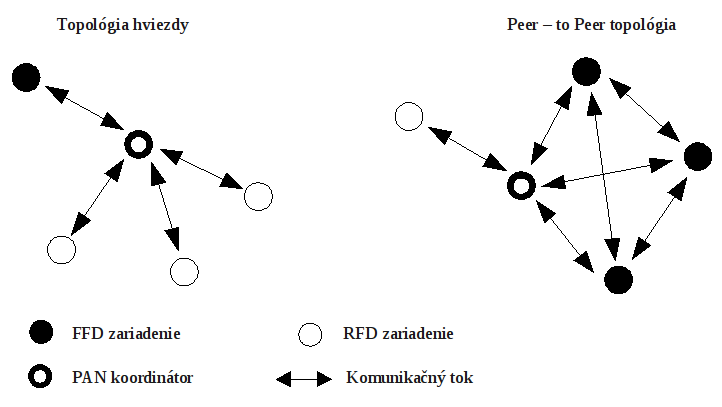
\includegraphics[width=12cm]{./figures/topologies802154.png}
 % topologies802154.png: 722x407 pixel, 72dpi, 25.47x14.36 cm, bb=0 0 722 407
 \caption{Topológie štandardu 802.15.4}
 \label{fig:80215topologies}
\end{figure}


\section{Architektúra}
Architektúra IEEE 802.15.4 viď. obrázok \ref{fig:802154layers} je tvorená pomocou vrstiev. Každá vrstva je zodpovedná za časť štandardu a poskytuje služby vyšším vrstvám. Vrstvy sú zavedené z dôvodu aby bol štandard ľahko popísateľný modelom ISO-OSI. 

LR-WPAN zariadenie je tvorené fyzickou vrstvou, ktorá zahŕňa rádiofrekvenčný vysielač, prijímač a mechanizmus potrebný na jeho obsluhu. Ďalšiu vrstvu tvorí linková vrstva, ktorá je zodpovedná za prístup všetkých prenosov ku komunikačnému kanálu. Jednotlivé vrstvy medzi sebou komunikujú pomocou prístupových bodov SAP (Service access point). Medzi vyššie vrstvy patrí sieťová vrstva a aplikačná vrstva, ktoré poskytujú zamýšľanú funkcionalitu zariadenia a patria do štandardu ZigBee. Architektúra LR-WPAN môže byť implementovaná u embeded zariadení a taktiež aj u zariadení vyžadujúcich pre svoj chod PC.

\subsection{Fyzická vrstva (PHY)}
Je zodpovedná za nasledujúce úlohy:
\begin{itemize}
\item aktivácia a deaktivácia rádiového vysielača a prijímača
\item detekcia energie na danom kanále
\item indikátor kvality spojenia (LQI – link quality indicator) pre prijaté rámce
\item výber frekvencie kanálu
\item príjem a odosielanie dát
\end{itemize}

Táto vrstva pracuje vo viacerých rádiových pásmách, konkrétne využíva 16 kanálov v pásme 2450 MHz, 30 kanálov v pásme 915 MHz a 3 kanály v pásme 868 MHz. Vysielač vysiela v následujúcich pásmach:
\begin{itemize}
\item 868-868.6 MHz (Európa)
\item 902-928 MHz (Severná Amerika)
\item 2400-2483.5 MHz (celosvetovo používané pásmo)
\end{itemize}

Prenosové rýchlosti prvého štandardu pre pásma s nižšou frekvenciou dosahovali hodnoty v rozsahu od 20 kb/s až do 40 kb/s, posledné pásmo bolo schopné pracovať s rýchlosťou až 250 kb/s. Novou verziou štandardu, za využitia modulácie signálu vo frekvenčnom pásme, boli zvýšené rýchlosti pásiem s nižšou frekvenciou na 100 až 250 kb/s.

\subsection{Linková vrstva (MAC)}
Plní následujúce úlohy:
\begin{itemize}
\item správa beacon rámcov (ich generovanie, synchronizácia)
\item prístup ku kanálu
\item GTS manažment
\item asociácia a disociácia PAN zariadení
\item bezpečnosť zariadení
\item riešenie kolízii na kanále metódou CSMA-CA
\end{itemize}

Beacon je špeciálny rámec, ktorý je vysielaný koordinátorom v pravidelných intervaloch, v prípade, že koordinátor má aktivovaný beacon mód. Tento rámec obsahuje napríklad informácie o konfigurácii sieti, bezpečnostné hlavičky, sekvenčné číslo rámca, pole použité k adresácii, GTS pole atď. Celý tento rámec sa následne vkladá do tela rámcov fyzickej vrstvy, pred ktorým stojí samotná hlavička fyzickej vrstvy.

\begin{figure}[h]
 \centering
 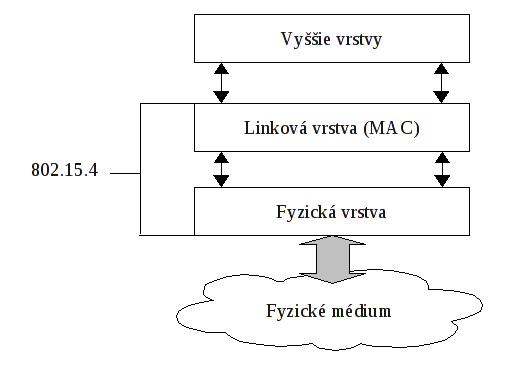
\includegraphics[width=10cm]{./figures/layers802154.png}
 % topologies802154.png: 722x407 pixel, 72dpi, 25.47x14.36 cm, bb=0 0 722 407
 \caption{Štruktúra štandardu 802.15.4}
 \label{fig:802154layers}
\end{figure}

\subsubsection{Typy rámcov}
Štruktúry rámcov boli navrhnuté aby zostala komplexnosť na minime, pri súčasnom zachovaní robustnosti pri posielaní dát na kanáli obsahujúcom šum.
Štandard definuje štyri druhy rámcov a to:
\begin{itemize}
\item beacon rámec
\item dátový rámec, ktorý sa používa pre prenos všetkých dát
\item potvrdzovací rámec, použitý k potvrdeniu úspešne prijatého rámca
\item MAC rámec, ktorý sa používa k spracovaniu všetkých servisných MAC prenosov
\end{itemize}

%TODO:
%?Režim spánku
%security page 24.

\chapter{Štandard ZigBee}
%ktorý zabezpečuje pre zariadenia, ktoré ho implementujú nízke náklady na ich výrobu, majú veľmi nízku spotrebuje energie,
Aliancia ZigBee stojí za vývojom komunikačného štandardu, ktorý je charakterizovaný nízkymi nákladmi na výrobu, nízkou spotrebou a bezpečnosťou u zariadení, ktoré ho implementujú. Samotný štandard vznikol v roku 2004 a jeho posledná revízia bola vykonaná v októbri 2007 (ZigBee-2007). Medzi hlavných členov ZigBee aliancie patria spoločnosti ako Motorola, Siemens, Atmel, Philips a iné. Tieto zariadenia nachádzali svoje hlavné uplatnenie v priemysle, no v dnešnej dobe, kde je snaha o digitalizáciu a automatizáciu ich môžeme ďalej nachádzať v konzumnej elektronike, zariadeniach pre medicínu, v automatizovanej domácnosti a budovách, pri riadení výrobných procesov a taktiež v rôznych senzorických zariadeniach. Zariadenia, ktoré chcú spĺňať ZigBee certifikáciu, musia napríklad vydržať pracovať so zdrojom energie - batériou minimálne po dobu dvoch rokov. ZigBee aliancia taktiež publikovala aplikačné profily, ktoré umožňujú vzájomnú komunikáciu medzi produktami aj napriek tomu, že sú od rôznych výrobcov (napríklad ZigBee Smart Energy).

%  čím sa redukuje ich dopad na environmentálne prostredia a zaraďujeme ich do triedy zariadení, ktoré sa nazývajú Smart Energy. 
\section{Architektúra}
Architektúra štandardu ZigBee je tvorená viacerými blokmi, ktoré nazývame vrstvy. Každá z vrstiev vykonáva špecifickú množinu operácii, ktoré následne využívajú nadradené vrstvy. Ďalej sú použité dátové jednotky, ktoré sú zodpovedné za prenos dát a riadiace jednotky vykonávajúce všetky ostatné služby. Každá jednotka poskytuje svoje funkcie vyšším vrstvám pomocou rozhrania, ktoré sa nazýva SAP. Každé SAP rozhranie poskytuje množstvo servisných primitív, pomocou ktorých sa dosahuje požadovaná funkcionalita.
ZigBee aliancia stavia na základoch štandardu IEEE 802.15.4-2003, ktorý definuje dve vrstvy a to fyzickú vrstvu (PHY) a spojovú vrstvu (MAC), viď. predošlá kapitola. Nadstavbu týchto vrstiev tvorí sieťová vrstva (NWK) a framework aplikačnej vrstvy. Tento framework je ďalej tvorený vrstvou APS (Aplication support sub-layer) a vrstvou nazývanou ZDO (ZigBee device objects). Špecifické aplikácie daných výrobcov následne využívajú daný framework, vrstvy APS a objekty ZDO. Samotná architektúra je zobrazená na obrázku \ref{fig:ZigBeeLayers}

\begin{figure}[h]
 \centering
 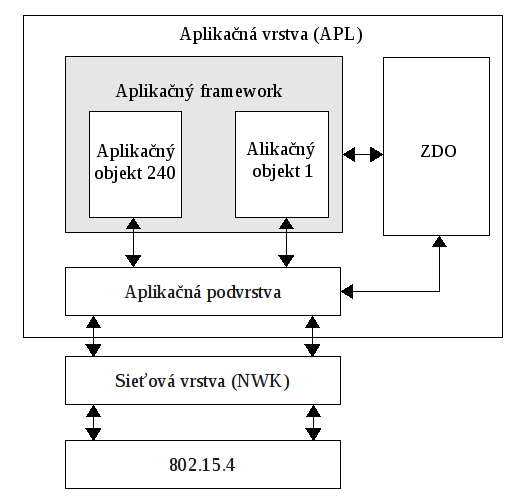
\includegraphics[width=10cm]{./figures/ZigBeeLayers.png}
 % topologies802154.png: 722x407 pixel, 72dpi, 25.47x14.36 cm, bb=0 0 722 407
 \caption{Štruktúra štandardu ZigBee}
 \label{fig:ZigBeeLayers}
\end{figure}

\section{Sieťové komponenty}
U sieti typu ZigBee rozoznávame nasledujúce tri druhy zariadení:
\begin{itemize}
\item ZigBee koordinátor, odpovedá PAN koordinátoru štandardu IEEE 802.15.4-2003
\item koncové zariadenie ZigBee, FFD alebo RFD zariadenie štandardu IEEE 802.15.4-2003, ktoré v ZigBee sieti nevystupuje ako ZigBee koordinátor alebo ZigBee smerovač
\item ZigBee smerovač, FFD zariadenie štandardu IEEE 802.15.4-2003, ktoré nemôže vystupovať v sieti ako ZigBee koordinátor, ale vystupuje ako koordinátor štandardu IEEE 802.15.4-2003, ktorý smeruje správy medzi zariadeniami a umožňuje asociáciu
\end{itemize}

\section{Sieťová topológia}
Sieťová vrstva štandardu ZigBee podporuje topológiu hviezda, ďalej stromovú a mesh (je to topológia používaná hlavne u bezdrôtových sieti, pri ktorej je každé sieťové zariadenie prepojené so všetkými ostatnými zariadeniami v danej sieti) topológiu.

\section{XBee Series 1}
Konkrétnu implementáciu predchádzajúcich štandardov tvoria moduly XBee/XBee PRO OEM od spoločnosti Digi, ktorá patrí do zoznamu certifikovaných výrobcov. V tejto práci som použil modul XBee Series 1, ktorý implementuje len štandard 802.15.4. Tento modul bol použitý pri meraniach v anténnej komore a jeho popisujúce parametre v samotnej simulácii. Linková vrstva modelu, ktorý som použil, pracovala s parametrami modulu TI CC1100, keď som chcel tieto parametre nahradiť, kontaktoval som spoločnosť Digi, ktorá mi však tieto parametre nebola schopná poskytnúť z dôvodu, že časť modulu, ktorá je zodpovedná za hodnoty týchto parametrov tvorí Ember 3.1 Stack, ktorý dodáva spoločnosť Ember. Spoločnosť Ember, však na moju žiadosť o sprístupnenie týchto parametrov (čas medzi prechodom z režimu spánku do režimu vysielania/prijímania, čas pri prechode zo stavu vysielania do stavu prijímania a opačne) vôbec nezareagovala.

\subsection{Technické parametre}
Modul popisujú následujúce parametre\cite{XBee}.

\begin{table}[htbp]
\begin{center}
\begin{tabular}{|c|c|}
\hline Dosah vnútri & 30m \\ 
\hline Dosah vonku & 90m \\ 
\hline Sila výstupného signálu & 1mW (0 dBm) \\
\hline Rýchlosť prenosu dát & 250 000 bps \\ 
\hline Rýchlosť sériového rozhrania & 1200 bps - 250 kbps \\ 
\hline Citlivosť pri príjme & -92 dBm \\
\hline 
\end{tabular} 
\end{center}
\caption{Špecifikácia výkonu a rýchlosti}
\label{tab:tab1}
\end{table}

\begin{table}[htbp]
\begin{center}
\begin{tabular}{|c|c|}
\hline Frekvenčné pásmo & ISM 2.4 GHz \\ 
\hline Rozmery & 2.438cm x 2.761cm \\ 
\hline Operačná teplota & -40 až 85C \\ 
\hline 
\end{tabular} 
\end{center}
\caption{Obecné parametre}
\label{tab:tab2}
\end{table}

\begin{table}[htbp]
\begin{center}
\begin{tabular}{|c|c|}
\hline Podporované sieťové technológie & Point-to-point, Point-to-multipoint, Peer-to-peer \\ 
\hline Počet kanálov & 16 \\ 
\hline Anténa & Whip \\
\hline Adresácia & PAN ID \\ 
\hline 
\end{tabular}
\end{center}
\caption{Sieťové parametre}
\label{tab:tab2}
\end{table}

\chapter{Teória antén}
Anténa je zariadenie, ktoré slúži na vysielanie a príjem rádiových signálov. Toto zariadenie konvertuje elektromagnetické vlny na elektrickú energiu a opačne. Podľa toho ako sú signály vysielané ich delíme na všesmerové (vysielanie vo všetkých smeroch) a smerové (vysielajú len v danom smere). Medzi chovaním sa vysielacej a prijímacej antény nepozorujeme žiadne rozdiely.

Následujúce parametre slúžia na popis základných vlastností antén:
\begin{itemize}
 \item smerovosť, určuje v akom smere sú elektromagnetické vlny vysielané. Je posudzovaná na základe vyžarovaných charakteristík, ktoré delíme na vertikálne a horizontálne. Meria sa pomocou parametrov zisk antény a vyžarovací uhol.
 \item vyžarovací uhol
 \item impedancia antény 
 \item zisk antény
 \item frekvenčná šírka prenášaného pásma
 \item polarizácia
 \item účinnosť
\end{itemize}

H rovina, je rovina v ktorej sa šíri vektor magnetického poľa a sleduje sa v nej ako sa mení intenzita elektrického poľa. Naopak v E rovine sa šíri vektor elektrického poľa a sleduje sa zmena intenzity magnetického poľa.

\subsection{Definícia pojmov}
Účinnosť je pomer vyžarovaného výkonu k výkonu, ktorý privádzame na vstup antény.
\linebreak 

\noindent Zisk určuje mieru smerovosti antény. Definujeme ho ako pomer vyžarovanej intenzity antény v danom smere k intenzite, ktorá je vyprodukovaná ideálnou anténou vyžarujúcou do všetkých smerov rovnomerne, bez strát a obe antény majú na vstupe rovnaký výkon. Zisk berie v úvahu okrem smerovosti aj účinnosť antény. Pre zisk ďalej platí, ak ma anténa pre daný smer väčší zisk ako je celkový zisk antény, tak v nejakom inom smere musí byť zasa zisk menší aby bola zachovaná celková energia. Tohoto faktu si je možno všimnúť u grafov popisujúcich zisk antén, ktoré boli vytvorené meraním v anténnej komore viď obrázok \ref{fig:xbeeWhipGain}.

%Relatívny zisk je pomer výkonového zisku pre daný smer k výkonovému zisku referenčnej antény vyžarujúcej v rovnakom smere. Vstupný výkon musí byť u oboch antén rovnaký. Referenčnou anténou je zvyčajne dipól alebo Horn anténa, u ktorých je hodnota vykonového zisku predom známa.

%Relative gain: The relative gain of a transmitting antenna in a given direction is defined as the ratio of the absolute gain of the antenna in the given direction to the absolute gain of a reference antenna in the same direction. The power input to the two antennas must be the same.

%smerovost = http://people.seas.harvard.edu/~jones/es151/prop_models/propagation.html#fsl

\subsection{Propagácia rádiového signálu}

Následujúci obrázok \ref{fig:RSP} zachytáva typický rádiový systém. Informácie vstupujú do vysielača. Informácie sú následne 
vysielané anténou, ktorá konvertuje rádiofrekvenčný signál na elektromagnetické vlny. Médium na prenos elektromagnetických vĺn je voľný priestor. Následne sú elektromagnetické vlny odchytené pomocou prijímacej antény, ktorá ich konvertuje spätne na rádiofrekvenčný signál. Ideálny stav je ak tento signál odpovedá signálu generovanému vysielačom. Originálna informácia, ktorá vstupovala do vysielača je následne demodulovaná na svoju pôvodnú formu.

\begin{figure}[h]
 \centering
 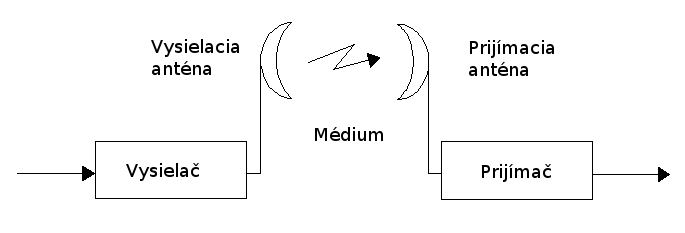
\includegraphics[width=10cm]{./figures/RSM.png}
 % topologies802154.png: 722x407 pixel, 72dpi, 25.47x14.36 cm, bb=0 0 722 407
 \caption{Model rádiového systému}
 \label{fig:RSP}
\end{figure}

\subsubsection{Pojmy}
\begin{itemize}
 \item dB - je skratka pre decibel. Je to matematické vyjadrenie používané na zobrazenie závislosti medzi dvoma hodnotami. 
 \item Rádiofrekvenčný výkon - je buď výkon vysielača alebo prijímača vyjadrený vo Wattoch. Taktiež môže byť vyjadrený v dBm. Vzťah medzi dBm a Wattmi je vyjadrený nasledovne $P_{dBm} = 10 * \log P_{mW}$
 \item Zoslabenie signálu modeluje nasledujúci obrázok \ref{fig:zoslab}. Kde Pin je vstupný výkon a Pout je hodnota výstupného výkonu.

 Zoslabenie je vyjadrené v dB podľa nasledujúceho vzťahu: $P_{dB} = 10 * \log(Pout / Pin)$. Napríklad predpokladajme, že dôjde k strate 1/3 vysielaného signálu (Pout/Pin = 2/3), potom hodnota zoslabenia v dB je 10 * log (2/3) = -4.05 dB
 
\item Citlivosť prijímača je minimálna hodnota výkonu radio frekvenčného signálu potrebná na vstupe prijímača, aby bol signál ďalej spracovaný. 

 \item Stratovosť je oslabenie výkonu radiofrekvenčneho signálu, ktorý je šírený v priestore. Je vyjadrená v dB a ďalej závisí na vzdialenosti medzi vysielacou a prijímacou anténou, na viditeľnosti medzi vysielacou a prijímacou anténou a na veľkosti antén.
\end{itemize}

\subsection{Typy antén}
\indent Izotropická anténa sa používa pre teoretické účely, vysielané vlny majú rovnaké parametre, ktoré popisujú anténu vo všetkých smeroch. Používa sa hlavne pri popisovaní a porovnávaní vlastností reálnych antén. 


\noindent Horn anténa sa používa v situácia, kde je potrebné dosiahnuť vysokého zisku, vlnová dĺžka je krátka, môže byť širokopásmová alebo úzko-pásmová, čo záleží na jej tvare. Taktiež dokáže pracovať s akoukoľvek frekvenciou. Keďže charakteristiky tejto antény sú známe a dobre matematicky popísané používa sa táto anténa ku kalibrácii iných systémov, tento fakt bol využitý aj počas meraní v anténnej komore. Hlavným parametrom, ktorý bol podstatný u meraní s touto anténou je jej zisk.


\noindent Whip anténa, je model antény, ktorý používajú ZigBee zariadenia, ktoré som simuloval. Anténa je poväčšine vertikálna a u ZigBee zariadení upevnená na doštičke plošného spoja. Je to anténa, ktorá vysiela horizontálne do všetkých smerov a hluché zóny sú vertikálne v bode upevnenia a ukončenia.

\subsection{Stratovosť voľného priestoru (Free-space path loss)}
%% http://www.radio-electronics.com/info/propagation/path-loss/free-space-formula-equation.php

Stratovosť signálu vo voľnom priestore sa používa k predikcii sily rádiového signálu. Napriek tomu, že nemodeluje dôveryhodne realitu obsahujúcu prekážky, odrazy atď, má veľký význam pre základné pochopenie šírenia sa signálu v reálnych podmienkach. Využíva sa taktiež pri tvorbe simulačných modelov a pri vývoji v oblasti bezdrôtových systémov.

Definujeme ju ako stratu sily signálu elektromagnetickej vlny, ktorá vzniká medzi dvoma priamo viditeľnými bodmi vo voľnom priestore, kde nie sú žiadne prekážky, odrazy a nedochádza k ohybu vĺn.

Formula pre výpočet stratovosti je nasledovná:
$$FSPL =  \left(\dfrac{4 \pi d}{\lambda}\right)^{2}  = \left(\dfrac{4 \pi d f}{c}\right)^{2},$$


kde:
\begin{itemize}
 \item $\lambda$ je vlnová dĺžka (m)
 \item f je frekvencia signálu (Hz)
 \item d je vzdialenosť od vysielača (m)
 \item c je rýchlosť svetla vo vákuu 2.99792458 * $10^{8}$ m/s
\end{itemize}

Daná formula vyjadrená v dB:

\begin{align*}
FSPL(dB) &= 10 \log_{10}\left(\dfrac{4 \pi df}{c} \right)^{2} \\
&= 20 \log_{10}\left(\dfrac{4 \pi df }{c} \right) \\
&= 20 \log_{10}(d) + 20 \log_{10}(f) + 20 \log_{10} \left(\dfrac{4 \pi}{c}\right)
\end{align*}


\subsection{Antény a simulácia}
Jednotlivé antény, na ktorých bolo vykonané meranie v anténne komore, boli popísané hodnotami výkonu (v dBm a W) v rozmedzí 0-360 stupňov pre každý stupeň. Z týchto hodnôt som pre každý stupeň spočítal hodnotu zisku. Samotný XML súbor, ktorý popisuje anténu a je použitý k simulácii potom obsahuje hodnoty ziskov po 10 stupňov, ktoré som spočítal ako priemer z hodnôt z meraní, čo samozrejme spôsobí ďalšiu odchýlku od reality. \\

%popis pocitania?


\begin{figure}[htbp]
 \centering
 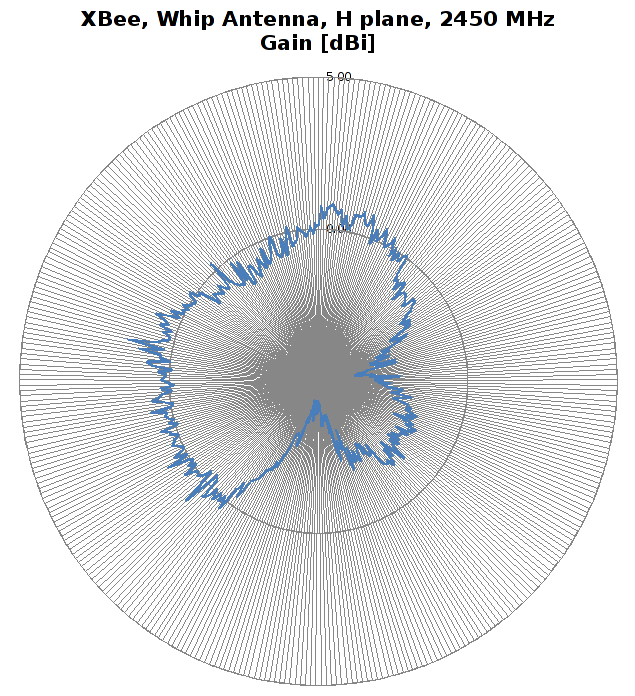
\includegraphics[width=9cm]{./figures/xbeeWhipGain.png}
 % topologies802154.png: 722x407 pixel, 72dpi, 25.47x14.36 cm, bb=0 0 722 407
 \caption{Charakteristika zisku antény Whip}
 \label{fig:xbeeWhipGain}
\end{figure}


\begin{figure}[htbp]
 \centering
 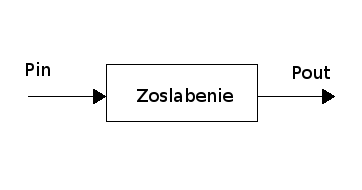
\includegraphics[width=8cm]{./figures/zoslabenie.png}
 % topologies802154.png: 722x407 pixel, 72dpi, 25.47x14.36 cm, bb=0 0 722 407
 \caption{Model zoslabenia signálu}
 \label{fig:zoslab}
\end{figure}


%%TODO:
%% 2 obrázky

\chapter{Simulátor OMNeT++}
OMNeT++ je objektový diskrétny simulátor\footnote{Je to systém kde zmeny stavu (udalosti) nastávajú v diskrétnych časových úsekoch a vykonanie udalosti netrvá žiaden čas.} napísaný v jazyku C++, využívajúci grafické prostredie (GUI), zameraný prevažne k simulácii komunikačných sieti, protokolov, softvérových a hardvérových architektúr. Celý nástroj spadá pod akademickú licenciu a tým pádom sa stáva voľne dostupný pre neziskové účely a jeho kód je taktiež verejne prístupný na Internete. Existuje aj komerčná verzia, ktorá sa nazýva OMNEST. Simulátor reprezentuje prístup na báze frameworku, namiesto toho aby poskytoval konkrétne komponenty špecifickej simulácie, čo umožňuje napríklad implementovať vlastný protokol bez nutnosti zásahu do jadra simulátoru. OMNeT++ je dostupný pre viacero platforiem a to Linux, Mac OS/X a Windows. Počas mojej práce som využil jeho inštaláciu na platforme Linux (Ubuntu). Na celom projekte sa zúčastňuje veľká komunita vývojárov a používateľov, programátorský a používateľský manuál \cite{OmnetApi}\cite{OmnetUser} je kvalitne spracovaný, taktiež existuje fórum a emailová skupina, ktorá je schopná zodpovedať mnohé otázky. Za povšimnutie stojí TicToc tutorial \cite{TicToc}, ktorý je vhodne preštudovať na úvod, pre pochopenie práce s danou simulačnou platformou.

V počiatkoch riešenia danej práce som začal pracovať s verziou OMNeT++ 3.2, no neskôr som prešiel na verziu OMNeT++ 4.0, ktorá sa stala medzitým stabilnou verziou. OMNeT++ 4.0 poskytuje vlastné vývojové IDE založené na aplikácii Eclipse. Oproti predchádzajúcej verzii došlo k viacerým zmenám, hlavne jazyk NED (Network Description) prešiel značnými zmenami. Simulácie môžeme spúšťať buď v grafickom prostredí Tkenv(Tcl/Tk) alebo z príkazovej riadky pomocou prostredia Cmdenv.

\subsection{Architektúra simulátoru}
OMNeT++ je tvorený simulačným jadrom a užívateľským prostredím. Simulačné jadro je zodpovedné za beh simulácie a obsahuje simulačnú knižnicu. Užívateľské rozhranie slúži pre spúšťanie, ladenie, demonštráciu a dávkové spúšťanie simulácie. Simulačnú knižnicu tvoria napríklad:
\begin{itemize}
\item generátor náhodných čísel
\item podpora smerovania v sieti a zisťovanie sieťovej topológie (trieda cTopology)
\item záznam štatistík do súboru (trieda cOutVector)
\item presmerovanie ladiacich výpisov do grafického prostredia (EV objekt)
\item správy
\end{itemize}

Keďže sa jedná o diskrétny simulátor, tak množina udalosti je reprezentovaná dátovou štruktúrou, ktorú nazývame FES (Future Event Set) alebo FEL (Future Event List). Prácu samotného simulátoru popisuje nasledujúci pseudokód:

%%%
\begin{verbatim}
inicializácia - vybudovanie modelu a vloženie prvých udalosti do FES

while(FES nie je prázdna a simulácia neskončila) 
{
	vyber prvú udalosť z FES
	t:= sprav časovú značku tejto udalosti
	spracuj udalosť
	(spracovanie udalosti môže pridať novú udalosť alebo zmazať existujúcu z FES)
}

ukončenie simulácie (zápis výsledkov, atď.)
\end{verbatim}
%%%

\subsection{Štruktúra modelu}
Simulovaný model v OMNeT++ je tvorený hierarchickou štruktúrou modulov, ktoré sa do seba môžu zanárať. Hĺbka ich zanorenia je neobmedzená. Moduly navzájom komunikujú pomocou správ, ktoré môžu byť tvorené komplexnými dátovými štruktúrami. Správy môžu reprezentovať v počítačových sietiach rámce, pakety, medzi modulmi sa predávajú pomocou brán. Každý modul môže obsahovať parametre, ktoré slúžia k predaniu konfiguračných dát do daného modulu, alebo definujú jeho topológiu. Parametre môžu byť následujúceho typu ako reťazec znakov, číslo, logická hodnota (áno, nie) alebo môžu byť popísané pomocou XML súboru. Štruktúra modelu je popísaná jazykom NED. Konfigurácia a vstupné dáta simulácie môžu byť ďalej popísané pomocou súboru omnetpp.ini alebo v NED súboroch. Samotnú funkcionalitu modulov tvoria metódy napísané v programovacom jazyku C++.


\subsection{Výstup simulácie}
Výsledky simulácii je možné zapisovať do súborov, ktoré môžme ďalej spracovať pomocou vizualizačných nástrojov. OMNeT++ rozlišuje dva spôsoby zápisu výstupných dát a to zápis pomocou vektorov alebo skalárov. Výstup v podobe vektorov obsahuje údaje, u ktorých má každý záznam pridelenú časovú značku, tento výstup je vhodný v prípade, že potrebujeme centrálny pohľad na danú simuláciu (je vhodný pre sledovanie vlastností typu spomalenie medzi koncovými bodmi, čas obehu paketov, stav fronty v danom čase). Vektory som použil na sledovanie hodnoty výkonu, ktorého hodnota sa menila so vzdialenosťou. Skaláry sú vhodné na sledovanie premenných, ktoré sa inicializujú na začiatku simulácie a po jej ukončení sa vyhodnotia. Použil som ich pre vyhodnocovanie výsledkov simulácie, konkrétne koľko rámcov bolo odoslaných a prijatých v prípade, že došlo k ich strate.

%% TODO
%% obrazok architektury omnetu ?? p235
%% spomenut ze moduly sa daju okrem rucnej konfiguracie cez NED modelovat aj pomocou grafickeho editoru NED
%% viacurovnova incializacia
%% popis suboru ANT

\chapter{Frameworky}
Samotný OMNeT++ neobsahuje žiadne moduly, ktoré by bolo možné použiť napríklad pre simuláciu bezdrôtovej siete. Konkrétne moduly pre dané simulácie sú implementované pomocou doplňujúcich frameworkov. Momentálne patria medzi hlavné sieťové simulačné modely frameworky Mobility Framework (MF) a INET Framework\cite{INET}. Popri ich vývoji vzniklo mnoho ďalších projektov ako napríklad LSU SenSim, Castalia, NesCT, MACSimulator, Positif, AdHocSim a iné. Vývoj mnohých z nich sa zastavil, poprípade zlúčil. Aktuálne najnovším sieťovým frameworkom je MiXiM\cite{MIXIM}, ktorý zlučuje MF a INET Framework. V tejto práci som použil MF, ktorý počas mojej práce prechádzal neustálymi zmenami, aktuálne sa stále nachádza v beta štádiu vývoja. Keďže som sa taktiež snažil zachovať aktuálnosť svojej aplikácie, moje výsledné úpravy MF odpovedajú aktuálne dostupnej verzii. V následujúcej časti popíšem vybrané frameworky a spomeniem ich hlavné vlastnosti, následne popíšem podrobnejšie architektúru MF, ktorý bol použitý.

\subsection{Mobility framework}
MF vnikol na univerzite Technische Universitaet Berlin, za cieľom poskytnúť kvalitnú základňu pre modelovanie bezdrôtových a mobilných sieti v simulátore OMNeT++. Prvotná verzia sa nazývala FraSiMO a práca na jej vývoji začala v roku 2001. Verzia, z ktorej vychádza aktuálny MF bola inicializovaná v roku 2003. Jadro frameworku implementuje podporu pre mobilitu uzlov, správu dynamických spojení a model kanálov u bezdrôtových sieti. Framework tvoria základné moduly, ktoré môžu byť ďalej ľahko použité pri implementácii vlastného protokolu. MF je možné použiť k simulácii nasledujúcich sieti:
\begin{itemize}
 \item nemobilné bezdrôtové siete
 \item mobilné bezdrôtové siete
 \item distribuované (ad-hoc) a centralizované siete
 \item senzorické siete
 \item viackanálové bezdrôtové siete
 \item iné simulácie, ktoré vyžadujú podporu mobility alebo rozhranie bezdrôtovej siete
\end{itemize}

Jeho aktuálna verzia, podporovaná simulátorom OMNeT++ 4, je v beta štádiu vývoja, pridáva implementáciu nasledujúcich modulov:
\begin{itemize}
 \item BatteryModule
 \item BMAC
 \item LMAC
 \item Rádiový model správy napájania ZigBee zariadení (TI CC 1100, TI CC 2420)
 \item štandard IEEE 802.15.4 CSMA (nepodporujúci beacon mód)
\end{itemize}


\subsection{INET Framework}
Tento framework vznikol z aplikácie IPSuite, ktorá bola vyvíjaná na Univerzite v Karlsruhe. INET Framework je open-source balík pre simulátory OMNeT++ a OMNEST, ktorý umožňuje simulovať sieťovú komunikáciu. Jeho aktuálna verzia podporuje následujúce Internetové protokoly: UDP, TCP, SCTP, IPv4, IPv6, Ethernet, PPP, IEEE 802.11, MPLS a iné. Taktiež nechýba podpora smerovacích protokolov ako OSPF.

Jeho podpora pre bezdrôtové a mobilných siete bola pôvodom prevzatá a modifikovaná z balíka MF. Daný framework som nepoužil pre riešenie mojej práce z dôvodu, že neobsahuje implementáciu štandardu IEEE 802.15.4, a jeho samotná implementácia by bola nad rámec tejto práce.

%??? modelovanie prostredia

\subsection{MiXiM}
Projekt MiXiM, ktorý bol iniciovaný v roku 2007, sa snaží zjednotiť aktuálne frameworky pre OMNeT++, s hlavným zameraním na mobilné a bezdrôtové simulácie. Jeho predchodcovia, z ktorých vychádza sú nasledujúce frameworky: ChSim, MacSimulator, Mobility Framework, Positif Framework. Jednou z najzaujímavejších vlastností toho projektu, je modelovanie reálneho prostredia, ktoré je v bezdrôtových sietiach zodpovedné za zmenu vysielaného signálu. K dispozícii je reálny 3D model prostredia, ďalej model stien a prekážok, ktoré obmedzujú mobilitu zariadení a tak spôsobujú zoslabenie vysielaného signálu, rôzne frekvencie a vysielacie média (rádiové vlny, ultrazvukové vlny), podpora multi-kanálov a iné. Súčasne pracuje s piatimi rozmermi a to 3D priestor, čas a frekvencia.

Aktuálne nebola stále uvoľnená žiadna oficiálna verzia projektu, čo je dôvodom, prečo nebol tento framework použitý pre moju prácu. K dispozícia sú zdrojové kódy, na ktorých vývoji sa neustále pracuje a jedným z hlavných nedostatkov je aktuálne chýbajúca dokumentácia. Architektúra \cite{MIXIMArch} tohoto frameworku, ktorá bola prezentovaná na posledom OMNeT++ seminári \cite{omnetWorkshop}, vyzerá veľmi zaujímavo a zdá sa, že bude kvalitným nástupcom aktuálnych frameworkov a súčasne prinesie mnoho zlepšení, vďaka, ktorým bude možné čoraz viac priblížiť simulácie bezdrôtových a mobilných zariadení reálnym podmienkam.



%\subsection{Iné} = Popis miletic a hallas a ine modely a preco som ich nepouzil
%Štandard IEE 802.15.4 implementuje viacero modelov. 


%*****************************************************************************
\chapter{Analýza a návrh riešenia}
%Analýza a návrh implementace (včetně diskuse různých alternativ a volby implementačního prostředí).

Práca sa snaží naviazať na predchádzajúce študentské práce, ktoré vznikli na fakulte (práca študenta U. Miletiča \cite{miletic} a B. Halása \cite{halas}) a boli zamerané na tému simulácii ZigBee sieti. Mojou snahou je priblížiť model simulácie ZigBee zariadení (na fakulte prebieha ich neustály výskum), konkrétne jeho časť definovanú štandardom IEEE 802.15.4, podporovanú Mobility frameworkom reálnym podmienkam, ktoré boli v mojom prípade popísané výsledkami meraní z anténnej komory.

Čo najdôveryhodnejšia simulácia bezdrôtovej komunikácie vyžaduje dokonalý model reálneho prostredia, rádiových kanálov a samotnej fyzickej vrstvy. Simulátory oboch predchádzajúcich študentských prác boli konštruované za účelom simulácie v ideálnych podmienkach (takzvané izotropné prostredie, kde nauvažujeme žiadne straty, rušenie a mobilitu zariadení). Modely teda vôbec nebrali v úvahu faktory prostredia a nauvažovali žiaden model antén, ktoré zariadenia využívajú pre vzájomnú komunikáciu. Takýto model simulácie však nie je uspokojujúci. K modelovaniu simulácie som zvolil MF, pretože predchádzajúce modely neboli jednak vhodne architektonicky navrhnuté pre podporu mobility a taktiež neimplementovali vhodnú funkcionalitu štandardu IEEE 802.15.4, u ktorého ma bude zaujímať hlavne fyzická vrstva.

\subsection{Model antén}
Model fyzickej vrstvy štandardu IEEE 802.15.4 v Mobility frameworku, implementuje šírenie sa rádiových signálov medzi bezdrôtovými zariadeniami bez akejkoľvek stratovosti. V mojej simulácii budem modelovať prenos týchto signálov za predpokladu, že celá komunikácia bude prebiehať vo voľnom priestore bez akýchkoľvek prekážok. Z toho vyplýva, že budem využívať formulu, z kapitoly zameranej na teoretické vlastnosti antén, určenú k výpočtu stratovosti signálu šírenom sa vo voľnom priestore (FSPL). Formula FSPL však nauvažuje žiadne faktory vzťahujúce sa k výkonu vysielača alebo zisku antén. V izotropnom prostredí platí, že hodnota výkonu privedeného na vstup vysielacej antény je rovná hodnote výkonu, ktorý dostaneme na výstupe z antény prijímacej. Pri prenose signálov vo voľnom priestore dochádza k ich oslabovaniu, čo spôsobuje, že prijímací výkon sa líši od vysielaného, tým že sa jeho hodnota znižuje. Na popis závislosti medzi výstupným a vstupným výkonom som použil formulu FSPL. V nasledujúcej časti textu odvodím daný vzťah medzi vysielacím a prijímacím výkonom pomocou formule FSPL a v ďalšej časti popíšem jeho samotnú implementáciu za pomoci využitia aplikácie MF.

%zmerat vstupne hodnoty vykonu na prijimaci??? 
Cieľom meraní v anténnej komore, bolo zmerať hodnoty výkonu u antén, ktoré používajú ZigBee zariadenia pre svoju vzájomnú komunikáciu. Meranie prebiehalo na prijímacej anténe typu Horn, ktorá mala fixnú polohu a bol známy jej zisk. Výsledná tabuľka meraní nachádzajúca sa v prílohe na CD udáva hodnotu výkonu v rozmedzí 0 až 360 stupňov, grafy zisku a výkonu pre jednotlivé antény. Z týchto hodnôt som následne spočítal zisk antén. Na daných grafoch je možné ďalej pozorovať, že zmenou výkonu vysielača pre konkrétnu anténu dochádza k zmene jej výkonovej charakteristiky no charakteristika zisku zostáva nezmenená. %TODO: preco? %
Pri počítaní zisku z výkonovej charakteristiky bol u jednotlivých antén, ktorými komunikovali ZigBee zariadenia použitý zisk Horn antény k normalizácii výsledných hodnôt. Na základe daného merania som dospel k záveru, že zisk antény má rôzne hodnoty v rôznych smeroch, následne som tieto hodnoty použil pre výpočet závislosti výstupného a vstupného výkonu.

\subsubsection{Výkonová závislosť}
%% http://en.wikipedia.org/wiki/Link_budget

Následujúci obrázok \ref{fig:FSPL} zobrazuje vysielač (T), u ktorého vystupuje dvojica výkonov $P_{1}$, $P_{2}$ a hodnota zisku pre daný smer $G_{T}(\alpha_{T})$, ďalej u prijímača (R) vystupujú výkony $P_{3}$, $P_{4}$ a zisk v danom smere $G_{R}(\alpha_{R})$. V simulácii bude zohrávať hlavnú úlohu hodnota výkonu $P_{4}$, hodnota výkonu $P_{1}$ je pred vyslaním rámcu známa, je to hodnota špecifikovaná výrobcom zariadenia. V následujúcej časti odvodím vzťah pomocou, ktorého určím hodnotu výkonu $P_{4}$, na základe ktorej sa prijímač rozhodne či sa naozaj jedná o prijímané dáta alebo sa vysielaný signál zoslabil na takú úroveň, kedy bude považovaný za šum na kanály.

Nasleduje formula pre výpočet hodnoty výkonu $P_{4}$, pomocou FSPL:

\[
\left[\frac{P_{3}}{P_{2}}\right]_{W} =\left(\frac{\lambda}{4\pi}\right)^{2}\frac{1}{d^{\alpha}}
\]

\begin{align*}
\left[\frac{P_{3}}{P_{2}}\right]_{dB} &= 10\log_{10}\left(\frac{\lambda}{4\pi}\right)^{2}\frac{1}{d^{\alpha}} \\
&= 10\log_{10}\left(\frac{c}{4\pi f}\right)^{2}\frac{1}{d^{\alpha}} \\
&= 20\log_{10}\left(\frac{c}{4\pi f}\right)-10\alpha\log_{10}d \\
&= -40.2251-10\alpha\log_{10}d, 
\end{align*}

kde:
\begin{itemize}
 \item $\lambda$ je vlnová dĺžka (m), $\lambda = \frac{c}{f}$
 \item f je frekvencia signálu (Hz), pre použité zariadenia XBee f = 2450 Mhz
 \item d je vzdialenosť od vysielača (m)
 \item c je rýchlosť svetla vo vákuu 2.99792458 * $10^{8}$ m/s
 \item $\alpha$ je koeficient útlmu prostredia (pre vzduch $\alpha = 2$)
\end{itemize}

Zavediem nasledujúce označenie:
$$L = -40.2251 - 10\alpha\log_{10}d$$

Ďalej platí:
\[
P_{2} = P_{1} + G_{T}(\alpha_{T}) \]
\[
P_{3} = P_{2} + L \]
\[
P_{4} = P_{3} + G_{R}(\alpha_{R}), \]

z čoho následne vyplýva následujúca rovnosť:
$$
P_{4} = P_{1} + G_{T}(\alpha_{T}) + G_{R}(\alpha_{R}) + L + K,
$$

kde:
\begin{itemize}
 \item $P_{1}$ - výkon privedený do antény vysielača (dBm)
 \item $P_{2}$ - výkon vysielaný vysielacou anténou (dBm)
 \item $P_{3}$ - hodnota výkonu prijatého prijímacou anténou (dBm)
 \item $P_{4}$ - výkon vystupujúci z káblu prijímacej antény a vstupujúci do prijímača (dBm)
 \item $G_{T}(\alpha_{T})$ - zisk vysielacej antény v danom smere (dBi)
 \item $G_{R}(\alpha_{R})$ - zisk prijímacej antény v danom smere (dBi)
 \item K - konštanta, ktorá spôsobuje ďalšie straty existujúce v reálnom prostredí (odrazy vo vodičoch, konektoroch, atď.)
\end{itemize}

Taktiež zároveň platí:
$$
P_{4}^{'} < P_{4}^{''},
$$

kde:
\begin{itemize}
 \item $P_{4}^{'}$ - hodnota výkonu v reálnom prostredí (W) 
 \item $P_{4}^{''}$ - spočítaná hodnota výkonu $P_{4}$ (W)
\end{itemize}

$$
\left[P_{3}\right]_{W} < \left[P_{2}\right]_{W} => \left[\frac{P_{3}}{P_{2}}\right]_{dB} < 0.
$$

Daný vzťah uvažuje straty, ktoré vznikajú na konektoroch antén, prepojovacím káblom medzi anténou a zariadením, vlastným odporom vodiča antény a iné. v podobe konštanty K.

%kedze model dokonalo modelujuci realne prostredie je zlozity... zameriame sa len na jeho cast ktorou v ktorej popiseme realne sa spravanie anten. anteny by boli uvazovane ze do vsetkych smeroch maju rovnaky zisk co je omyl... doplnenie modelu MiXmiX nasim realnym popisom anten bude o to realistickejsie.
%teoria k tomu ako sa riesi simulacia realneho prostredia 
%Rádio frekvenčné signály sa prenášajú veľmi rýchlo, no počas ich prenosu môže dochádzať k ich strate poprípade odrazom.

\begin{figure}[htbp]
 \centering
 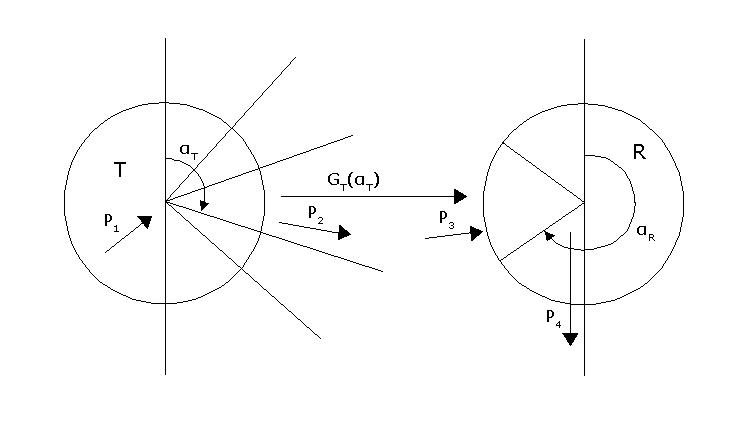
\includegraphics[width=10cm]{./figures/FSPL.png}
 % topologies802154.png: 722x407 pixel, 72dpi, 25.47x14.36 cm, bb=0 0 722 407
 \caption{Popis výkonov a zisku u antén pre vysielač a prijímač}
 \label{fig:FSPL}
\end{figure}


\subsection{Štruktúra MF}
V tejto časti sa zameriam na detailný popis funkcie modulov a ich následnú implementáciu. Obrázok \ref{fig:Host} zachytáva štruktúru stanice, ktorú popisujeme pomocou jazyka NED. Na základe konvencie musí názov súboru vo svojom názve obsahovať reťazec \uv{host}. Ako môžeme vidieť daná stanica sa skladá z jednotlivých podmodulov a to aplikačná vrstva, sieťová vrstva a vrstva NIC, ktoré navzájom komunikujú. Stanica taktiež obsahuje modul \textit{Mobility}, ktorý zabezpečuje pohyb a geografickú pozíciu uzlu. 

Podmoduly modulu stanica majú spoločného predka, ktorým je trieda \textit{BasicModule}. Táto trieda je ďalej potomkom triedy \textit{cSimpleModule}, ktorá je súčasťou Omnetu. Trieda \textit{BasicModule}, obsahuje dvojfázovú inicializáciu, ktorá je vhodná aj v prípade použitia modulu \textit{Blackbox} \footnote{Je to modul umožňujúci medzivrstvovú komunikáciu, bez nutnosti zasielania správ}, ktorý v tomto texte nebudem popisovať. Medzi ďalšie vlastnosti patrí napríklad metóda \textit{logName}, ktorá vracia názov NED modulu, čo je možné využiť pri ladení za pomoci makra EV, ktoré slúži pre výpis ladiacich správ. 

Samotná komunikácia medzi jednotlivými podmodulmi modulu stanice je zabezpečená pomocou metód:
\begin{itemize}
 \item \textit{handleUpperMsg} - táto metóda je volaná zakaždým, keď modul obdrží správu z vyššej vrstvy, následne ju spracuje a predá nižšej vrstve
 \item \textit{handleLowerMsg} - metóda je volaná po príchode správy z nižšej vrstvy, správu ďalej spracuje a predá nadradenej vrstve
\end{itemize}

Ďalej sú k dispozícii pomocné metódy slúžiace k enkapsulácii a dekapsulácii správy predávanej medzi vrstvami (\textit{encapsMsg, decapsMsg}) a metódy na opozdenie správy pri jej vysielaní na kanál.

Keďže model poskytuje enkapsuláciu a dekapsuláciu správ, z toho vyplýva, že pre každú vrstvu definujeme osobitný typ správy, ktorej štruktúra je popísaná pomocou súboru s príponou .msg. K dispozícii sú napríklad správy typu \textit{AirFrame} (správa pre komunikáciu na fyzickej vrstve), \textit{MacPkt} (správa pre komunikáciu na linkovej vrstve), \textit{NtwPkt} (správa pre sieťovú vrstvu) a \textit{ApplPkt} (správa pre vrstvu aplikačnú). Všetky typy správ sú rozšíriteľné, resp. si pomocou nich môžeme odvodiť vlastný typ správy. Pre potreby mojej simulácie bola najdôležitejšia správa typu \textit{AirFrameRadioAccNoise3}, zdedená z triedy \textit{AirFrame}, ktorej štruktúra obsahuje následujúce položky

\begin{itemize}
 \item pSend - výkon, ktorým bol rámec odoslaný
 \item channelId - kanál, na ktorý bola správa zaslaná
 \item duration - čas, ktorý bol spotrebovaný na zaslanie rámcu (v sekundách)
 \item hostMode - štruktúra popisujúca pozíciu stanice, jej rýchlosť, smer pohybu, čas kedy sa pohyb začal
 \item SnrControlInfo - trieda, ktorá obsahuje pomocné informácie SNR (Signal to noise ratio), ktoré sa predávajú modulu \textit{Decider}
\end{itemize}

%snr infor z MSG decideru a z nich spocitame bit errors

Danú správu som ďalej rozšíril o parameter moduleId, ktorý obsahuje globálny identifikátor modulu, z ktorého bola správa odoslaná.

\begin{figure}[h]
 \centering
 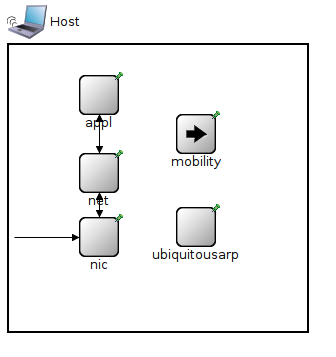
\includegraphics[width=6cm]{./figures/host.png}
 % topologies802154.png: 722x407 pixel, 72dpi, 25.47x14.36 cm, bb=0 0 722 407
 \caption{Štruktúra stanice v OMNeT++}
 \label{fig:Host}
\end{figure}

\subsubsection{Štruktúra modulu NIC}

%% finut tie pojmy  ,, mac vrstva == spojova ?
NIC (Network card interface) je časť sieťového adaptéru zodpovedná za fyzický prístup k médiu a adresácii na úrovni MAC vrstvy, popisuje ju fyzická a linková vrstva ISO-OSI modelu. Štruktúra tohoto modulu je znázornená na obrázku \ref{fig:Nic}. V mojom prípade je teda fyzická vrstva tvorená modulom \textit{snrEval}, \textit{decider} a vrstvu MAC tvorí modul \textit{mac}. Vzájomná úzka kooperácia medzi týmito vrstvami je dôvodom prečo sú zapuzdrené v jednom module. Všetky submoduly modulu NIC, sú zdedené z triedy \textit{ChannelAcces}, ktorá je ďalej odvodená z triedy \textit{BasicModule}. Táto trieda poskytuje funkcionalitu umožňujúcu komunikáciu jednotlivých staníc, ktoré sú vo vzájomnom dosahu. Na úrovni fyzickej vrstvy ma hlavne zaujíma modelovanie oslabenia signálu a výpočet chybovosti na kanále. Tým, že je fyzická vrstva tvorená osobitne modulom \textit{snrEval}, som schopný modelovať výpočet stratovosti na kanále pomocou rôznych metód a na základe výsledku sa v module \textit{decider} rozhodnem pomocou akého kritéria tieto dáta vyhodnotím. Napríklad modul \textit{decider} bude rozhodovať o tom či dané dáta príjme na základe porovnania hodnoty SNR, spočítanej z modulu \textit{snrEval}, s definovanou hraničnou hodnotou, alebo sa môže rozhodovať na základe počítania pomocou formúl pre výpočet chybovosti na kanále (napr. BER). Vďaka tomu môžem tieto moduly navzájom rôzne kombinovať. V následujúcej časti detailnejšie priblížim štruktúru modulov \textit{snrEval} a \textit{decider}. \\


\noindent\textbf{Modul snrEval}

Tento modul zabezpečuje príjem a vysielanie dát na kanál. Ďalej vytvára správy typu \textit{AirFrame} z \textit{MacFramu} a opačne, počas toho ako odpočúva kanál zároveň mení stavy rádia, ktoré sú reprezentované stavovým automatom a taktiež zabezpečuje simuláciu oneskorenia vo vysielaní alebo príjme pomocou pomocných funkcií (\textit{bufferMsg, unbuefferMsg}). V mojom modele ma zaujímala jedna z jeho ďalších vlastností a to ukladanie a spracúvanie SNR hodnôt pri prijímaní rámcov. Rámec fyzickej vrstvy (\textit{AirFrame}) obsahuje pomocnú štruktúru \textit{SnrList}, ktorú reprezentuje štruktúra \textit{List} programovacieho jazyka C++ a záznam tejto štruktúry obsahuje dve položky a to časovú značku prijatia rámcu a k nej odpovedajúcu hodnotu SNR. V mojom prípade je hodnota SNR spočítaná na základe vzťahu [hodnota výkonu vstupujúca do prijímača ($P_{4}$) / hodnota šumu na kanále], kde hodnotu $P_{4}$ počítam za využitia modifikovanej formule FSPL. Túto hodnotu následne predávam do modulu \textit{Decider}, kde je ďalej spracovaná.

Práca modulu snrEval je znázornená vývojovým diagramom na obrázku \ref{fig:snrEval}. Keď sa nachádza modul v stave SYNC prijíma správu. Pred jej prijatím sa najskôr vykoná kontrola, či nedošlo k poškodeniu SFD (Start frame delimiter), následne sa spracuje zvyšok správy a spočíta sa hodnota SNR. V prípade, že sa modul nenachádza v stave SYNC a obdrží ďalšiu správu je tato správa považovaná za šum, hodnota šumu sa zvýši o hodnotu výkonu, ktorým bola táto správa prijatá a spočíta sa nová hodnota SNR, ku ktorej je pripojená časová značka. Detailnejšie sa budem zaoberať modelom kolízie v následujúcej kapitole.

%% rcdPower / noiseLevel

V tomto module je metóda \textit{handleLowerMsg} rozdelená na dve časti a to:
\begin{itemize}
 \item \textit{handleLowerMsgStart} - volá sa hneď po prijatí správy, volá metódy na výpočet hodnoty prijatého výkonu ($P_4$) a následne predáva spracovanie ďalším metódam na základe stavu rádia
 \item \textit{handleLowerMsgEnd} - slúži na samotné odoslanie správy vyššej vrstve a zároveň pripája \textit{SnrList} ako parameter.
\end{itemize}


\noindent\textbf{Modul decider}
 
Modul spracúva len správy, ktoré prichádzajú z kanálu cez modul \textit{SnrEval}. Správy z vyšších vrstiev, ktoré sa posielajú na kanál neprechádzajú týmto modulom a to z dôvodu, že tento modul len rozhoduje, či sa daná správa zahodí alebo prepošle vyššej vrstve. Rozhodovanie je založené na základe výpočtov ako napríklad chybovosť bitov alebo sa rozhoduje či sa má správa zahodiť na základe vysokej hodnoty šumu na kanále porovnaním s hraničnou hodnotou. Tieto vlastnosti však sledujem len u správ prichádzajúcich z kanálu. \textit{Decider} teda slúži na výpočet chybných bitov (BER) v správe, čo počíta pomocou hodnôt uložených v štruktúre \textit{SnrList}. Ďalej je v ňom možné implementovať rôzne opravné kódy. V simulácii je použitý vzorec na výpočet chybných bitov (BER) pre moduláciu MSK. 
$$BER = 0.5 * exp(-0.5 * SNR)$$


Modul \textit{mac} ďalej poskytuje funkcionalitu metódy na riadenie prístupu k médiu CSMA. Modul \textit{radio} je centrálne zdieľaný a moduly ako \textit{snrEval} alebo \textit{mac} prepínajú jeho stavy (napr. RX, TX) podľa potreby. Posledným modulom, je modul \textit{antenna} ktorý popisuje parametre antény a je využívaný modulom \textit{snrEval}.

%\subsubsection{Mobiná architektúra a správa komunikačného kanálu} 

\begin{figure}[h]
 \centering
 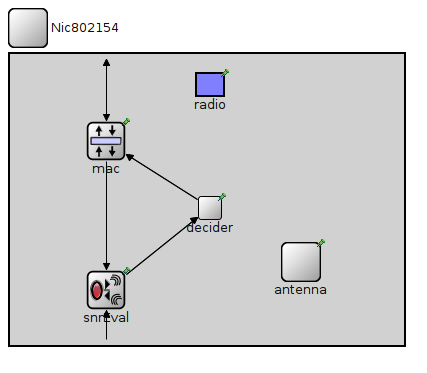
\includegraphics[width=8cm]{./figures/nic.png}
 % topologies802154.png: 722x407 pixel, 72dpi, 25.47x14.36 cm, bb=0 0 722 407
 \caption{Štruktúra NIC v OMNeT++}
 \label{fig:Nic}
\end{figure}

\begin{figure}[h]
 \centering
 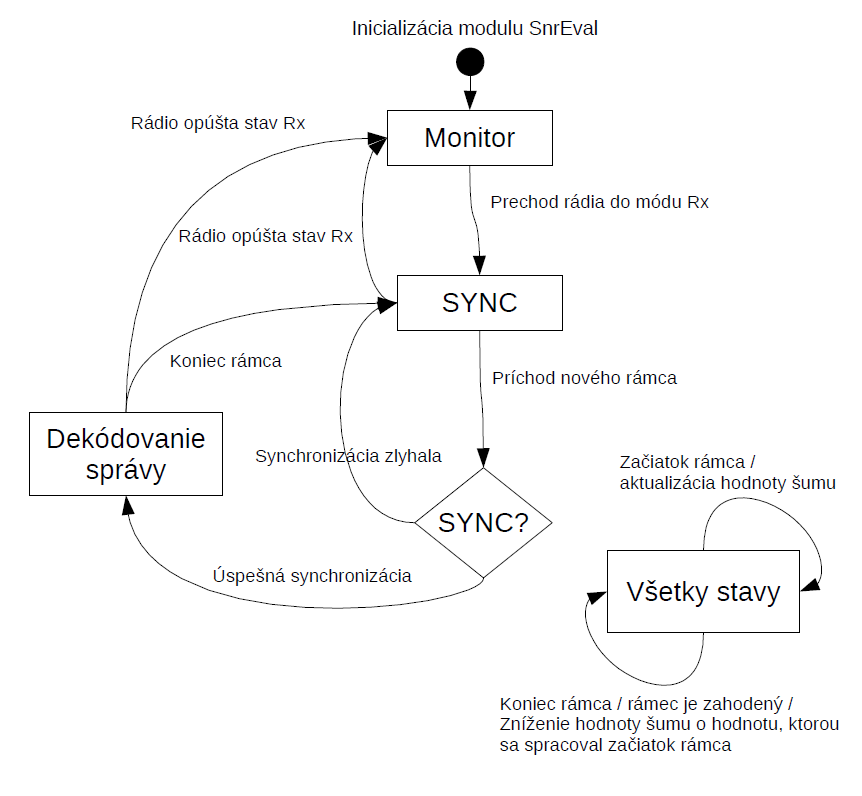
\includegraphics[width=13cm]{./figures/snrEval.png}
 % topologies802154.png: 722x407 pixel, 72dpi, 25.47x14.36 cm, bb=0 0 722 407
 \caption{Prechody medzi stavmi v module snrEval}
 \label{fig:snrEval}
\end{figure}

%*****************************************************************************
\chapter{Realizácia}

Pre potrebu simulácie som teda ako prvý vytvoril modul \textit{Antenna}, ktorý popisuje anténu ZigBee zariadení následujúcimi parametrami:
\begin{itemize}
 \item zisk - ideálny zisk antény, ktorý nájdeme v popise antény (dBi)
 \item impedancia ($\Omega$)
 \item config - odkazuje na xml súbor popisujúci zisk antény (*.xml)
\end{itemize}

Modul sa snaží byť čo najobecnejší pre prípadne využitie aj v iných modeloch a pridal som ho medzi ostatné moduly MF. Z predošlých parametrov je najdôležitejší parameter \textit{config}. Pomocou tohoto parametru sa odkazujem na súbor, ktorým popisujem zisk antény pre daný uhol, v ktorom anténa prijíma alebo vysiela. Hodnoty tohoto súboru sú z meraní, ktoré boli vykonané v anténnej komore. Nasledujúce riadky zachytávajú príklad popisu konkrétnej antény. 

\begin{verbatim}
<?xml version="1.0" encoding="UTF-8"?>
<!DOCTYPE antenna SYSTEM "Antenna.dtd">
<antenna>
        <angle min="0" max="0" gain="0.3" />
        <angle min="0" max="30" gain="0.4" />
        <angle min="30" max="360" gain="0.9" />
<antenna>
\end{verbatim}

Jednotlivé záznamy v elementoch <angle ...>, reprezentujú hodnotu zisku pre uhol z intervalu (min, max>. Jednotlivé intervaly musia byť zoradené vzostupne, bez prekrývania sa. V prípade, že je rámec odoslaný pod uhlom ktorý, sa v popisnom xml súbore nenachádza, je použitá  hodnota ideálneho zisku, ktorá je zapísaná v .ned súbore popisujúcom štruktúru modulu antény. Táto hodnota môže byť prepísaná v konfiguračnom súbore danej simulácie omnetpp.ini pomocou nasledujúceho zápisu: 
sim.host[*].nic.antenna.gain = 2.1dBi

Parametru \textit{config}, ktorý odkazuje na xml súbor je potrebné priradiť xml súbor aj v prípade ak chcem v simulácii použiť len hodnotu teoretického zisku antény. V aktuálnej verzii Omnetu nie je možné priradiť tomuto parametru napríklad hodnotu \uv{false} a zabezpečiť týmto neodkazovanie sa na xml súbor. Túto funkcionalitu som ďalej do Omnetu neimplementoval, pretože po konzultácii s autorom Omnetu, som sa dozvedel, že táto možnosť pribudne v jeho novej verzii. Tento prípad riešim tak, že parametru config priradím xml súbor obsahujúci samotný koreňový element <root />, ktorý vyhodnotím pri samotnom spracúvaní xml súboru.

Samotný xml súbor popisujúci konkrétny model antény priradím danej stanici následovne: sim.host[*].nic.antenna.config = xmldoc(\uv{antenna1.xml})

%validuje???
Po spustení simulácie sa v inicializačnej časti modulu validuje daný xml súbor pomocou súboru Antenna.dtd, ďalej sa načíta do pamäti, z dôvodu, že simulátor poskytuje len DOM parsér a sprístupním si odkaz na jeho prvý element <angle ...>. Modul ďalej obsahuje metódu \textit{findGainValue}, ktorá v danom xml súbore vyhľadá hodnotu zisku pre daný uhol. Z dôvodu optimalizácie som pre vyhľadávanie v štruktúre xml súboru použil binárne vyhľadávanie.

Ďalej som do modulu \textit{SnrEvalRadioAccNoise3} implementoval výpočet modifikovanej formule FSPL. Samotný priestor, takzvaný playground, v ktorom sa odohráva simulácia som rozdelil na štyri kvadranty, vďaka čomu dokážem veľmi efektívne počítať uhol, pod ktorým bol rámec vyslaný z vysielacej stanice a uhol, pod ktorým bol rámec prijatý na prijímacej stanici. Tieto uhly sú prepočítané na strane príjemcu, z ich hodnôt zistím pomocou modulu antény, konkrétne hodnoty daných ziskov $G_{T}(\alpha_{T})$ a $G_{R}(\alpha_{R})$. Hodnotu zisku $G_{R}(\alpha_{R})$ určím priamo pomocou metódy \textit{faindGainValue} modulu \textit{antenna}, ktorý obsahuje prijímač. Prijatý rámec obsahuje hodnotu jedinečného identifikátoru modulu (moduleId), z ktorého bol vyslaný. Pomocou neho sprístupním odkaz na modul vysielača a taktiež zavolám jeho metódu \textit{findGainValue}, ktorá mi vráti hodnotu zisku $G_{T}(\alpha_{T})$. Následne môžem spočítať hodnotu výkonu $P_4$, z tejto hodnoty sa ďalej spočíta hodnota SNR pomocou vzťahu SNR = $P_4$/[hodnota šumu prostredia], kde hodnota šumu prostredia je rovná -100dBm. SNR sa ďalej pripojí ako kontrolná informácia k rámcu a odošle o úroveň vyššie vrstve \textit{decider}. Táto vrstva následne spočíta hodnotu BER pre daný rámec a v prípade, že nedošlo k poškodeniu rámca je tento rámec predaný opäť vyššej vrstve a to vrstve MAC.

Pre potreby vyhodnocovania modelov, som ďalej upravil modul \textit{ChannelControl}, kde bol pridaný parameter ratio, pomocou, ktorého je prepočítavaná vzdialenosť v modeli na reálnu vzdialenosť.

Počas implementácie a ladenia modelu som objavil v produkčnom kóde MF, dve chyby, konkrétne pri výpočte hodnoty BER v module \textit{decider}, druhá chyba bola v module \textit{snrEval}. Po upozornení autora boli obe chyby opravené.

% Popis vrstvy APPL layer
%V mojom prípade som v module snrEval zmenil a pridal to a to
%??? a v module decider som pouzit - pridal - zmenil to a to.

%kolizia.png

\subsection{Model kolízie}
Pri komunikácii ZigBee zariadení v reálnom prostredí môže dochádzať k ich vzájomnému rušeniu. Takáto situácia môže nastať napríklad v prípade, že nastane kolízia v mechanizme, ktorý riadi prístup k médiu (CSMA-CA) alebo ak máme dve siete, kde prijímač z prvej siete príme súčasne v jednom okamihu počas svojho stavu Rx, dva rámce. Súčasné prijatie dvoch rámcov na anténe zanesie do komunikácie šum (čo je vlastne prídavný signál), ktorý môže ďalej spôsobiť chybovosť (BER). Keďže, som chcel modelovať aj situácie, u ktorých by dochádzalo k rušeniu, musel som pre tieto potreby model čiastočne modifikovať. Daný model neposkytuje vrstvy štandardu ZigBee preto nie je možné modelovať dve nezávislé siete. Danú kolíziu som preto vytvoril pomocou modifikácie MAC vrstvy, čím som dosiahol, že dané zariadenie sa chovalo ako generátor šumu, tj. periodicky vysiela rámce, s tým, že dochádza ku kolízii a prijímač príjme viacero rámcov súčasne.

V simulácii je používaný diskrétny simulátor, počas simulačného času prebiehajú udalosti. Model súčasného prijatia viacerých rámcov vyzerá tak, že v čase keď prijímač príjme rámce simulačný čas sa zastaví a samotné prijatie rámcov považujeme za udalosti v rovnakom simulačnom čase. Procesorový čas však neustále beží a teda program obsluhujúci súčasne prijatie viacerých rámcov príjme tieto rámce v skutočnosti s určitým časovým odstupom, čo je v simulácii reprezentované pomocou udalosti. Najprv je prijatý prvý rámec, je spracovaná jeho obsluha, následne sa spracuje druhý rámec atď. Tomuto popisu odpovedá nasledujúci obrázok \ref{fig:kolizia}, ktorý zachytáva situáciu pri ktorej došlo ku kolízii v modifikovanej vrstve MAC (modul \textit{mac}).

\subsubsection{Popis kolízie}
Obrázok \ref{fig:kolizia} je výstup z nástroja Sequence chart a detailný popis jednotlivých udalosti je možné analyzovať pomocou nástroja Event log. Oba tieto nástroje sú vhodné pre analýzu simulácie poprípade jej ladenie a pribudli vo verzii OMNeT++ 4.0. V mojom modely \ref{fig:modelKolizie} som simuloval vznik kolízie na module host[0], ktorý periodicky prijímal rámce z modulu host[1]. Modul host[2] som použil ako generátor rámcov, ktoré budú spôsobovať kolízie. Na obrázku reprezentuje sivý úsek zastavenie simulačného času. Modul host[0] prijal v rovnaký čas dva rámce, prvý od modulu host[1], čomu odpovedá číslo udalosti 41, druhý od modulu host[2] s číslom udalosti 43. Oba tieto rámce boli prijaté modulom \textit{snrEval}. Na základe predchádzajúceho popisu modulu \textit{snrEval}, prebehne následujúca obsluha:
\begin{enumerate}
 \item rámec z udalosti 41, vstupuje do modulu \textit{snrEval}, ktorý sa sa prepne do stavu SYNC, keďže sa jedná o nový rámec, je spočítaná hodnota SNR1, nasleduje prepnutie do stavu Dekódovanie správy \\ \\
 SNR1 = (výkon, ktorým bol rámec prijatý / šum)
 \item následne je prijatý rámec z udalosti 43, tento rámec bude spracúvaný ako šum, spočíta sa nová hodnota SNR2, rámec sa následne zahodí \\ \\
 SNR2 = (hodnota výkonu, ktorým bol prijatý rámec z udalosti 41) / (šum + prijatý výkon rámca z udalosti 43)
 \item ukončí sa spracovanie rámca z udalosti 41, hodnoty SNR1 a SNR2 sa pripoja ako kontrolné informácie k správe, ktorá sa následne prepošle modulu \textit{decider}
 \item \textit{decider} na základe hodnôt SNR1, SNR2 spočíta BER a podľa jeho hodnoty sa rozhodne či sa rámec zahodí (tj. rámec obsahuje chybné bity) alebo pošle modulu \textit{mac}
\end{enumerate}

Čím je nižšia hodnota SNR, tým je vyššia pravdepodobnosť, že prijatý rámec bude obsahovať chyby. Tento fakt vychádza zo Shannonovej vety, danej nasledujúcou formulou, ktorá udáva max. teoretický limit prenosovej rýchlosti C kanálu s pásmom o šírke W a odstupom signálu od šumu (SNR).

$$ C = W * \log_{2} (1 + SNR) [b/s, Hz] $$

V prípade, že sa hodnota SNR blíži k nule, prenosová rýchlosť kanálu sa taktiež blíži k nule, z čoho vyplýva, že dochádza k veľkej strate prenášaných dát, čo zapríčiní veľkú chybovosť na prenášaných dátach. \\

\begin{figure}[h]
 \centering
 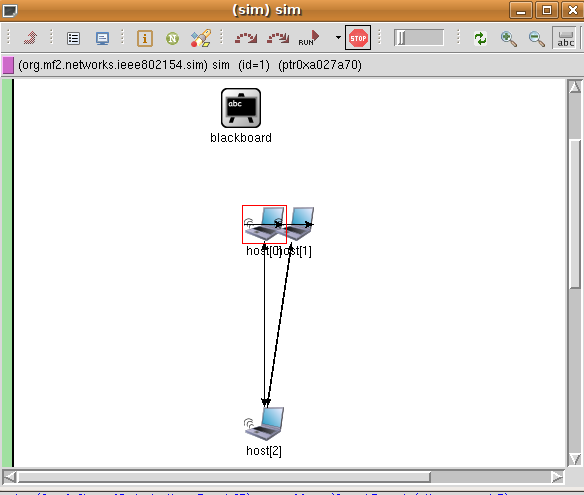
\includegraphics[width=10cm]{./figures/modelKolizie.png}
 % topologies802154.png: 722x407 pixel, 72dpi, 25.47x14.36 cm, bb=0 0 722 407
 \caption{Model kolízie}
 \label{fig:modelKolizie}
\end{figure}

\begin{figure}[h]
 \centering
 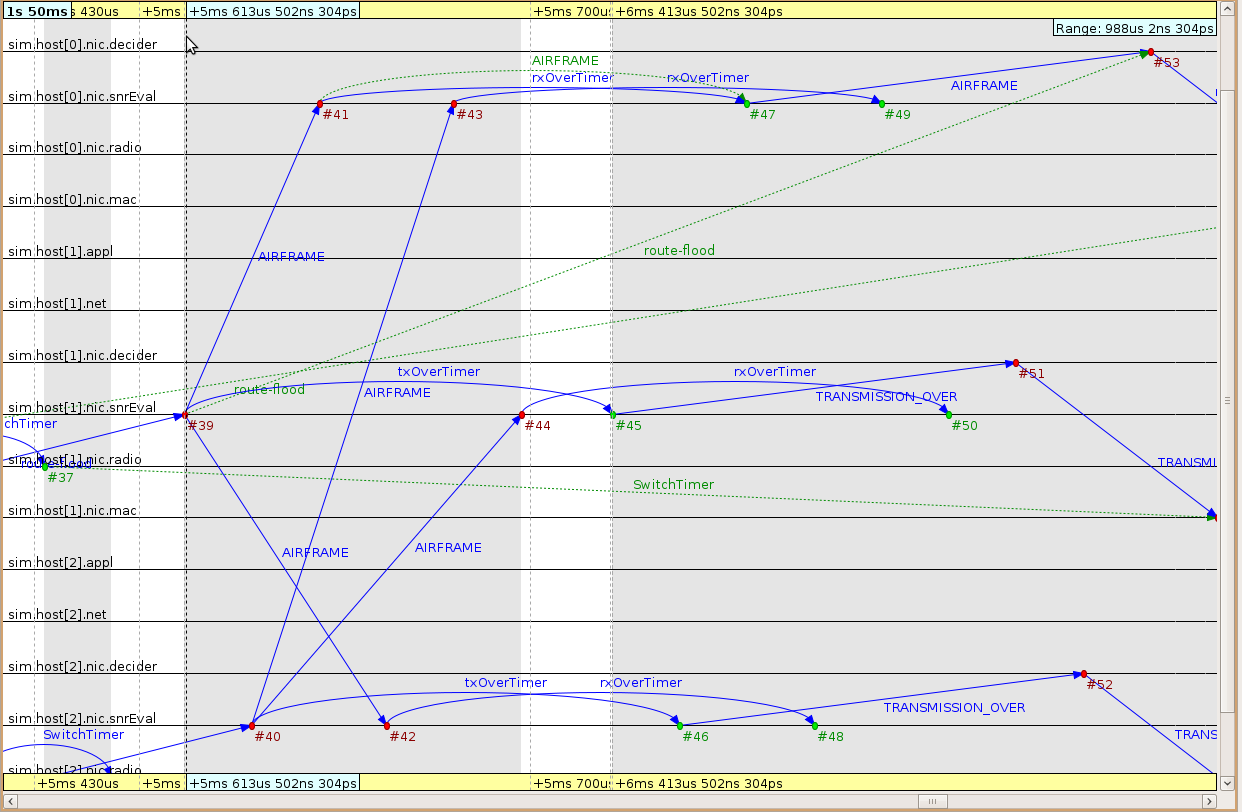
\includegraphics[angle=90, width=15cm]{./figures/kolizia.png}
 % topologies802154.png: 722x407 pixel, 72dpi, 25.47x14.36 cm, bb=0 0 722 407
 \caption{Kolízia na MAC vrstve}
 \label{fig:kolizia}
\end{figure}

%*****************************************************************************
\chapter{Testovanie}

V tejto časti popíšem testy, ktoré som uskutočnil pomocou daného modelu a porovnám výsledky týchto testov s reálnym meraním.

\subsection{Testy zamerané na pohyb XBee zariadení}
Pri vykonávaní týchto testov, som modeloval komunikáciu dvoch XBee zariadení, z ktorých jedno bolo v pozícii príjemcu a vysielač sa pohyboval. Hlavný faktor, na ktorý som kládol dôraz bolo pozorovanie ako sa mení hodnota výkonu na strane príjemcu s narastajúcou vzdialenosťou. Taktiež som sledoval počet zahodených rámcov, takzvanú stratovosť rámcov (na základe výpočtu chybovosti BER na prijímači) s narastajúcou vzdialenosťou a oslabovaním sa signálu, viď tabuľka \ref{tab:stratovost1} \\

Vykonal som následujúce testy:
\begin{enumerate}
 \item vzdiaľovanie sa vysielača (s výkonom vysielača 1mW a 10mW) po kroku 0.6cm (po každom kroku bol vyslaný rámec) do vzdialenosti 5m, viď. grafy \ref{fig:5m-1mW} a \ref{fig:5m-10mW}
 \item vzdiaľovanie sa vysielača (s výkonom vysielania 1mW a 10mW) po kroku 0.6cm (po každom kroku bol vyslaný rámec) do vzdialenosti 5m a súčasná náhodná rotácia oboch zariadení okolo vlastnej osi
 \item vzdiaľovanie sa vysielača (s výkonom vysielania 1mW  a 10mW) po kroku 0.6m (po každom kroku bol vyslaný rámec) do vzdialenosti 250m, viď. graf  \ref{fig:250m-10mW}
 \item vzdiaľovanie sa vysielača (s výkonom vysielania 1mW  a 10mW) po kroku 0.6m (po každom kroku bol vyslaný rámec) do vzdialenosti 250m a súčasná náhodná rotácia oboch zariadení okolo vlastnej osi, viď. graf \ref{fig:250m-1mW-rotace}
 \item náhodná rotácia vysielača okolo prijímača vo fixnej vzdialenosti 10m
\end{enumerate}

Detailné výstupy z týchto testov sa nachádzajú na priloženom CD vo forme spracovaných grafov a taktiež vo forme súboru s príponou .sca, čo je jeden z výstupných formátov simulátoru Omnet, ktorý sa dá ďalej vhodne spracúvať pomocou nástroja Scave.

%Grafy z merani

%Grafy z realu
Analýzou týchto meraní je vidno, že krivky grafov sa takmer zhodujú s reálnymi meraniami a to aj napriek tomu, že reálne prostredie obsahuje množstvo faktorov spôsobujúcich odrazy atď. Daným modelom som schopný modelovať reálne podmienky s vysokou presnosťou aj napriek tomu, že zanedbám straty, ktoré v nich vznikajú.

\begin{table}[htbp]
\begin{center}
\begin{tabular}{|c|c|c|}
\hline Vzdialenosť [m] & Stratovosť [\%] & Výkon vysielača [mW]\\ 
\hline 100 & 0 & 1\\ 
\hline 150 & 0.12 & 1\\ 
\hline 200 & 11.87 & 1\\ 
\hline 220 & 30.42 & 1\\ 
\hline 250 & 76.38 & 1\\
\hline 300 & 49.65 & 10\\  
\hline 
\end{tabular} 
\end{center}
\caption{Stratovosť rámcov}
\label{tab:stratovost1}
\end{table}

\subsection{Testy s kolíziou}
V týchto testoch bola poloha zariadení XBee stacionárna. Model uvažoval dve zariadenia prijímač a vysielač, kde vysielač vysielal rámce. Ďalej som do simulácie zapojil generátor šumu (zariadenie periodicky generujúce rámce, ktoré spôsobovali kolíziu). V tejto simulácii som sledoval koľko rámcov bolo zahodených (stratovosť) z dôvodu šumu spôsobeného generátormi na prijímači. \\

Vykonal som následujúce testy:
\begin{enumerate}
 \item model viď. obrázok \ref{fig:modelKolizie} prijímač - host[0], vysielač - host[1] boli umiestnené vo vzdialenosti 30cm, generátor šumu - host[2] (vysielací výkon 10mW) vo vzdialenosti 3m a 4m
 \item model totožný s predchádzajúcim no bol pridaný druhý generátor šumu, jeho umiestnenie bolo x = host[2].x - 0.7m, y = host[2].y. Vysielací výkon oboch generátorov šumu bol 10mW. 
\end{enumerate}

\begin{table}[htbp]
\begin{center}
\begin{tabular}{|c|c|c|}
\hline Vzdialenosť generátora šumu [m] & Stratovosť [\%] & Stratovosť v reálnych podmienkach [\%]\\ 
\hline 3 & 9.8 &15\\ 
\hline 4 & 0 & nebolo merané\\ 
\hline 
\end{tabular} 
\end{center}
\caption{Prípad č. 1}
\label{tab:stratovost2}
\end{table}

\begin{table}[htbp]
\begin{center}
\begin{tabular}{|c|c|}
\hline Vzdialenosť generátorov šumu [m] & Stratovosť [\%] \\ 
\hline 3 & 98\\ 
\hline 4 & 80\\ 
\hline 
\end{tabular} 
\end{center}
\caption{Prípad č. 2}
\label{tab:stratovost3}
\end{table}
%tabulka


%vyhodnotenie ???

\begin{figure}[htbp]
 \centering
 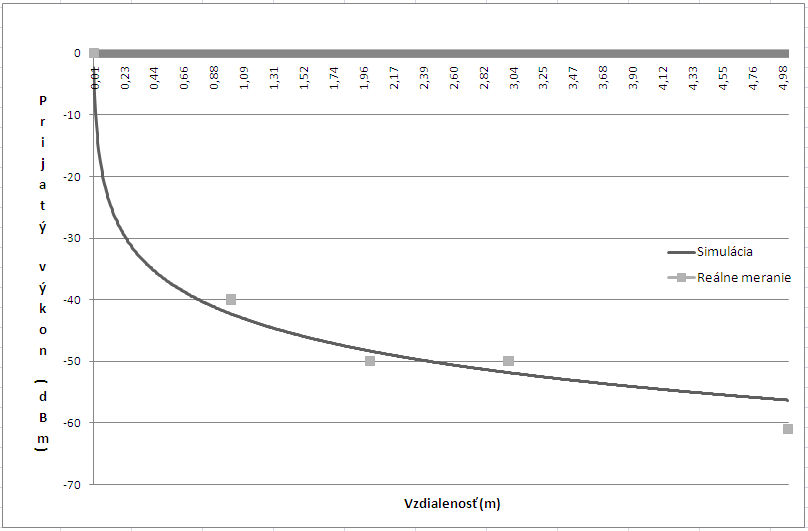
\includegraphics[width=13cm]{./figures/results/5m-1mw.png}
 % topologies802154.png: 722x407 pixel, 72dpi, 25.47x14.36 cm, bb=0 0 722 407
 \caption{Pohyb na vzdialenosť 5m, vysielací výkon 1mW}
 \label{fig:5m-1mW}
\end{figure}

\begin{figure}[htbp]
 \centering
 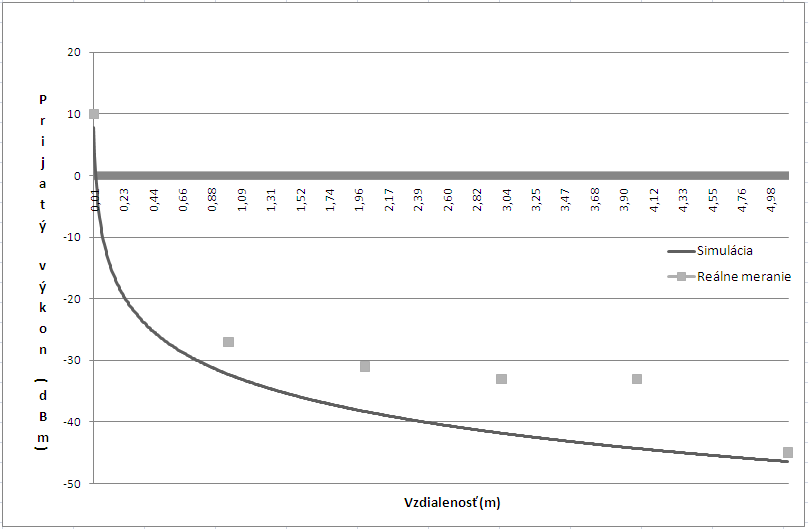
\includegraphics[width=13cm]{./figures/results/5m-10mw.png}
 % topologies802154.png: 722x407 pixel, 72dpi, 25.47x14.36 cm, bb=0 0 722 407
 \caption{Pohyb na vzdialenosť 5m, vysielací výkon 10mW}
 \label{fig:5m-10mW}
\end{figure}

\begin{figure}[htbp]
 \centering
 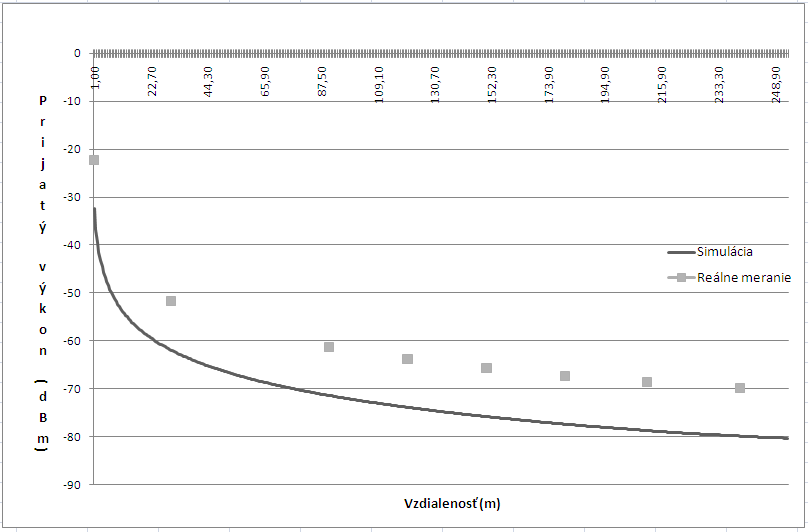
\includegraphics[width=13cm]{./figures/results/250-10mw.png}
 % topologies802154.png: 722x407 pixel, 72dpi, 25.47x14.36 cm, bb=0 0 722 407
 \caption{Pohyb na vzdialenosť 250m, vysielací výkon 10mW}
 \label{fig:250m-10mW}
\end{figure}

\begin{figure}[htbp]
 \centering
 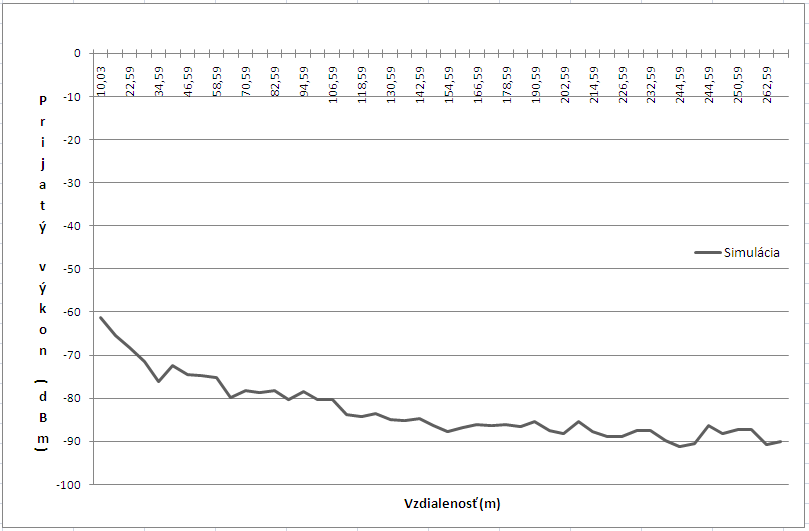
\includegraphics[width=13cm]{./figures/results/250-1mw-rotace.png}
 % topologies802154.png: 722x407 pixel, 72dpi, 25.47x14.36 cm, bb=0 0 722 407
 \caption{Pohyb na vzdialenosť 250m, vysielací výkon 1mW, rotácia okolo vlastnej osi}
 \label{fig:250m-1mW-rotace}
\end{figure}


%*****************************************************************************
\chapter{Záver}

Práca na tejto téme bola plná úskalí, ktoré sa mi na jej konci podarilo úspešne prekonať. Počas jej spracúvania som sa oboznámil s relatívne mladým štandardom IEEE 802.15.4 a technológiou ZigBee, ktorá ho využíva. Ďalej som sa oboznámil a vyskúšal si prácu so simulátorom OMNeT++, ktorý je v dnešnej dobe značne využívaný akademickou ale aj komerčnou sférou. V začiatkoch práce som pracoval s jeho staršou verziou 3.x, no neskôr som prešiel na verziu 4.0, ktorá sa medzičasom stala stabilnou a priniesla mnoho výhod, ktoré boli zužitkované pri simulovaní modelu, spracúvaní výsledkov a ladení simulácie. Po teoretickej stránke som sa oboznámil s mnohými vlastnosťami antén a zákonmi, ktoré platia pri prenose signálu u bezdrôtových zariadení. Dúfam, že sa mi podarí poznatky v tejto problematike naďalej prehlbovať.

Jednou z najťažších úloh bola práca s Mobility frameworkom, ktorý disponuje nepostačujúcou dokumentáciou, počas práce sa neustále vyvíjal a aktuálne sa stále nachádza v beta štádiu. Z toho dôvodu som sa v analýze práce zameral aj na detailný popis funkcie modulov, ktoré som využíval a neboli vôbec zdokumentované. Bohužiaľ po analýze Miletičovej práce nebolo možné naviazať na jeho model z dôvodov kódovej nekompatibility na vyššiu verziu Omnetu a nevhodnej architektúre modelu pre podporu mobility. Implementácia antén do toho frameworku sa úspešne podarila a taktiež bol úspešne zrealizovaný celý model, ktorým som následne bol schopný simulovať fyzickú vrstvu ZigBee zariadení v reálnych podmienkach, ktoré boli popísané na základe výstupov z reálnych meraní. Modelom som dokázal simulovať útlm signálu na základe vzdialenosti a chybovosť rámcov, ktorú som modeloval pomocou generátora šumu. Počas analýzy kódu Mobility frameworku sa mi podarilo odhaliť dve chyby, ktoré boli následne po upovedomení autora opravené v produkčnom kóde.

Paralelne počas písania mojej práce, prebiehala na fakulte diplomová práca zameraná na tvorbu modelu, ktorý bude simulovať vrstvy patriace ZigBee štandardu. Architektonicky sú obe práce pripravené na vzájomné prepojenie, čo môže byť vhodným podnetom na ďalšie pokračovanie a spojenie týchto práci v kvalitný simulátor ZigBee zariadení.


%\item Zhodnocení splnění cílů DP/BP a  vlastního přínosu práce (při formulaci je třeba vzít v potaz zadání práce).
%\item Diskuse dalšího možného pokračování práce.

%*****************************************************************************
% Seznam literatury je v samostatnem souboru reference.bib. Ten
% upravte dle vlastnich potreb, potom zpracujte (a do textu
% zapracujte) pomoci prikazu bibtex a nasledne pdflatex (nebo
% latex). Druhy z nich alespon 2x, aby se poresily odkazy.

\bibliographystyle{abbrv}
%bibliographystyle{plain}
%\bibliographystyle{psc}
{
%JZ: 11.12.2008 Kdo chce mit v techto ukazkovych odkazech take odkaz na CSTeX:
\def\CS{$\cal C\kern-0.1667em\lower.5ex\hbox{$\cal S$}\kern-0.075em $}
\bibliography{reference}
}

% M. Dušek radi:
%\bibliographystyle{alpha}
% kdy citace ma tvar [AutorRok] (napriklad [Cook97]). Sice to asi neni  podle ceske normy (BTW BibTeX stejne neodpovida ceske norme), ale je to nejprehlednejsi.
% 3.5.2009 JZ polemizuje: BibTeX neobvinujte, napiste a poskytnete nam styl (.bst) splnujici citacni normu CSN/ISO.

%*****************************************************************************
%*****************************************************************************
\appendix


%*****************************************************************************
\chapter{Zoznam použitých skratiek}

\begin{description}
\item[APL] Aplication Layer
\item[APS] Aplication Support Sub-layer
\item[CSMA-CA] Carrier Sense Multiple Access - Collision Avoidance
\item[FFD] Full Functionality DEvice
\item[FEL] Future Event List
\item[FES] Future Event Set
\item[FSPL] Free-space path loss
\item[GTS] Guaranteed Time Slot
\item[GUI] Graphical User Interface
\item[IDE] Integrated Development Environment
\item[LQI] Link Quality Indicator
\item[LR-WPAN] Low-Rate Wireless Personal Area Network
\item[MAC] Medium Access Control
\item[MF] Mobility Framework
\item[NED] Network Description
\item[NIC] Network Card Interface
\item[NWK] Network
\item[RFD] Reduced Functionality Device
\item[PAN] Person Area Network
\item[PHY] Physical
\item[SAP] Service Access Point
\item[SFD] Start Frame Delimiter
\item[SNR] Signal to noise ratio
\item[ZDO] ZigBee Device Object
\item[WLAN] Wireless Local Area Network
\item[WPAN] Wireless Personal Area Network
\end{description}


%*****************************************************************************
\chapter{Inštalačná a užívateľská príručka}

\subsection{Inštalácia simulátoru OMNeT++ pre platformu Linux}
\begin{enumerate}
 \item Stiahnutie archívu obsahujúceho zdrojový kód zo stránok \\
 \url{http://www.omnetpp.org/omnetpp}
 \item Prekopírovanie archívu do adresára /usr/local/
 \item Rozbalenie archívu pomocou príkazu tar zxvf omnetpp-4.0.src.tgz
 \item Do užívateľského profilu .bash\_profile alebo .profile pridáme riadok \\
  export PATH=\$PATH:/usr/local/omnetpp-4.0/bin
  \item Je potreba zabezpečiť prítomnosť následujúcich balíkov v systéme 
    \begin{tabbing}
    sudo apt-get install \= build-essential gcc g++ bison flex perl tcl8.4 tcl8.4-dev \\
                       \> tk8.4 tk8.4-dev blt blt-dev libxml2 libxml2-dev \\
                       \> zlib1g zlib1g-dev libx11-dev
    \end{tabbing}    
 \item Prevedieme následujúce príkazy: \\
   cd /usr/local/ometpp-4.0 \\
   ./configure \\
   ./make
 \item Spustenie OMNeT++ s IDE pomocou príkazu omnetpp 
\end{enumerate}

\subsection{Inštalácia mnou modifikovaného Mobility Frameworku}
\begin{enumerate}
 \item Stiahnutie súborov Mobility frameworku z svn http://my-svn.assembla.com/svn/mframework/, poprípade prekopírovanie adresára mf2o4 z priloženého CD do adresára /usr/local/
 \item Import MF do aplikácie OMNeT++
  \begin{enumerate}
   \item Po spustení aplikácie Omnet, klikneme na oblasť \uv{Project explorer}, pravým tlačítkom a zvolíme položku \uv{Import...}
   \item Zvolíme \uv{General->Existing project into Workspace}
   \item V položke \uv{Select root directory}, zvolíme cestu k adresáru mf2o4, tj. /usr/local/mf2o4
   \item Pomocou CTRL+B, preložíme zdrojové súbory
  \end{enumerate}  
\end{enumerate}

\subsection{Práca s modelom IEEE 802.15.4}
Vo vývojom prostredí Omnetu si otvoríme v oblasti \uv{Project explorer} adresárovú štruktúru mf2o4, kde si následne otvoríme adresár networks a v ňom adresár ieee802.15.4. V tomto adresári sa nachádzajú aj xml súbory popisujúce antény. Otvoríme si súbor omnetpp.ini, tento súbor je hlavným konfiguračným súborom modelu simulácie. Zahrnul som do neho ukážkové nastavenia viacerých modelov, ktoré som simuloval. Samotná simulácia sa potom spustí otvorením súboru omnetpp.ini a následným kliknutím na tlačítko \uv{Run} z menu aplikácie.

%*****************************************************************************
\chapter{Obsah priloženého CD}

Následujúci obrázok \ref{fig:zoznamCD} zobrazuje štruktúru priloženého CD.

\begin{figure}[h]
\begin{center}
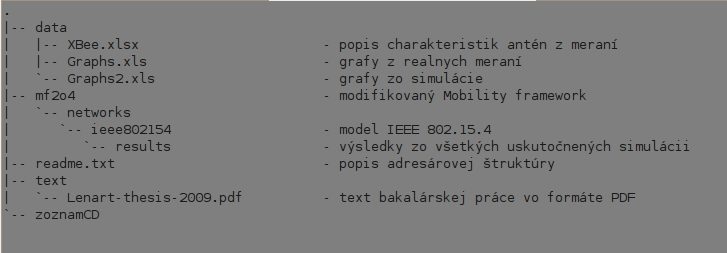
\includegraphics[width=14cm]{./figures/zoznamCD.png}
\caption{Výpis priloženého CD}
\label{fig:zoznamCD}
\end{center}
\end{figure}

\end{document}
